\cotefile{18}
\scanpage{18}
A - 20 - \hfill n° 413

(resp. $U_n(\underline V)$) et ses éléments seront appelés \uline{distributions} (resp. \uline{distributions d'ordre} $\leq n$) sur $\underline V$. La restriction $\varphi_*$ à $U(\underline V)$ du transposé de $\varphi^*$ est donc un isomorphisme de modules filtrés de $U(\underline V)$ sur $S(M)$ et permet de transporter à $U(\underline V)$ la structure de coalgèbre avec forme unité de $S(M)$ : la prop. 6 montre que la structure de coalgèbre obtenue est indépendante de la carte choisie et la multiplication dans $\widehat P(\underline V)$ (qui s'identifie au dual de $U(\underline V)$) est la transposée de l'application diagonale de $U(\underline V)$. On désignera par $U_+(\underline V)$ le noyau de la forme unité ; c'est aussi l'image réciproque par $\varphi_*$ du sous-module $\displaystyle\sum_{k>0}S^k(M)$. On appellera \uline{module tangent} à $V$ et on notera $T(\underline V)$ l'intersection $U_+(\underline V)\cap U_1(\underline V)$ : c'est aussi l'image réciproque de $M=S^1(M)$ par $\varphi_*$.

Si $f\in\widehat P_+(\underline V;\underline V')$, le transposé de $f^*$ envoie $U(\underline V)$ dans $U(\underline V')$. Sa restriction à $U(\underline V)$ sera notée $f_*$. C'est une application linéaire compatible avec les filtrations, avec les structures de coalgèbres avec forme unité. La restriction de $f_*$ à $T(\underline V)$ est une application linéaire de $T(\underline V)$ dans $T(\underline V')$ appelée \uline{application linéaire tangente à} $f$ et notée $T(f)$ : si $\underline V$ et $\underline V'$ sont les noyaux formels définis par des modules $M$ et $M'$, cette définition est en accord avec celle donnée au n° 1, à condition d'identifier $T(M)$ et $M$ (et $T(M')$ avec $M'$) ce qui est loisible.

Supposons maintenant que $\underline V'$ soit le noyau formel associé à un module libre $M$. On peut alors à $\underline u\in\widehat P_+(\underline V;M)$ associer la composée de $\underline u_*$ et de la projection canonique de $S(M)$ sur $S^1(M)=M$ : on obtient ainsi un isomorphisme de $\widehat P_+(\underline V;M)$ sur le sous-module de $\operatorname{Hom}(U(\underline V);M)$ formé des applications linéaires nulles sur $U_0(\underline V)$ (il suffit pour le voir de prendre une carte de $\underline V$ et d'utiliser la remarque 2 du n° 4). Pour tout module séparé $N$, nous pouvons définir une application formelle

\margin{\mspage{\unsure{17}}}

\scanpage{19}
Soit $X$ un \unsure{schém.} algébrique lisse sur \deleted{\unsure{$k$}} un corps $k$ isomorphe à $\mathbf C$ [de façon non précisée]. Alors
\diagram{\begin{tikzcd}[ampersand replacement=\&]
 A^p(X) \arrow[r,"P_{\mathrm{alg}}"] \& \underline{\underline H}^{2p}(X,\Omega_X^\bullet)
\end{tikzcd}}
est bien défini. Le choix d'un isom $\sigma$ $k\xleftarrow{\sim}\mathbf C$ fixé permet de définir
\margin{\unsure{cano} = \uline{De Rham} + \uline{\unsure{Gr.}}}
\diagram{\begin{tikzcd}[ampersand replacement=\&]
 P_\sigma^{(p)}:\quad A^p(X) \arrow[r,"{\unsure{\mathrm{cano}}\,\unsure{P_{\mathrm{top}}^{an}}\;\deleted{\unsure{P_\sigma^{an}}}}"] \& \underline{\underline H}^{2p}(X,\Omega_X^\bullet)
\end{tikzcd}}
qui se factorise par un sous-réseau $E_\sigma^{\unsure{2i|2p}}=H^{2p}(X_\sigma,\mathbf Z)$ de $\underline{\underline H}^{2p}(X,\Omega_X^\bullet)$. On a
\[
 P_\sigma^{(p)}=\left(\frac{1}{\sigma(2i\pi)}\right)^p P_{\mathrm{alg}},
\]
ce qui montre que $P_\sigma^{(p)}$ dépend beaucoup de $\sigma$, \inserted{$\pi$ étant \uline{transcendant}}. Dans le cas où
\diagram{\begin{tikzcd}[ampersand replacement=\&]
 A^p(X) \arrow[r,"P_\sigma^{(p)}","\unsure{\sim}"'] \& H^{2p}(X_\sigma,\mathbf Z)
\end{tikzcd}}
est un isom (ex: $p=1$, $X=\mathbf P^1$) on voit de $\unsure{=}$ que le réseau $E_\sigma^{\unsure{2i|2p}}$, égal à $\displaystyle\frac{1}{\sigma(2i\pi)}P_{\mathrm{alg}}(A^p(X))$, dépend beaucoup de $\sigma$. \uline{NB} \unsure{Remplaçant} $\sigma$ par $\bar\sigma$ change $P_\sigma^{(p)}$ en $-P_\sigma^{(p)}$, donc ne change pas les $E_\sigma^i=H^{\unsure{2i|i}}(X_\sigma,\mathbf Z)$

\mspage{18}

\scanpage{20}
SYSTÈMES de RACINES (15) \hfill Tribu n° 59

\uline{n° 5} - Identifier $V'$ à son dual à la p. 195. A la p. 196 décrire plus explicitement $P(R)$ et $Q(R)$ : $Q(R)=L_0\cap V'$, $P(R)$ est la proj. orthogonale de $L_0$ sur $V'$, (cf. résultat ajouté au § 6, n° 8) ; on a $P=Q+Zv'$ où $v'$ est la projection de $(1,0,\ldots,0)$, (on a $(\ell+1)v'=(\ell,-1,\ldots,-1)$.

En bas de la p. 196, ne pas identifier tout de suite $W$ et le groupe d'autom. de $R^{\ell+1}$ d'où il peut venir, mais remonter $W$ en un groupe $G$ ; déterminer $S(R^{\ell+1})$, $S(R^{\ell+1})^G$, $S(V')$ et $S(V')^W$. Diviser par la factorielle à la l.15, p. 197.

Dans (XI) dire, tout de go, que l'autom. échange $i$ et $\ell-i+1$. Ajouter l'effet de $\operatorname{Aut}(R)$ sur $P/Q$.

\uline{n° 6} - Prendre $\ell\geq1$... Pas de dual à la p. 199. Dire seulement que $\gamma=(4\ell-2)(\ell+1)$, en référant à la formule (13)...
Dans (IX) et (X) dire que $W(R)$ se compose des applic. linéaires telles que... ; c'est seulement un produit semi-direct. Diviser par la factorielle dans (7), p. 201. Remplacer ``Etant'' par ``Comme ils sont'', (p. 201, l.6). Ce qu'on dit dans (XI) concerne le cas $\ell\geq2$ ; ajouter que la même conclusion est évidente pour $\ell=1$.

\uline{n° 7} - Prendre $\ell\geq1$. Parler de ``base'' d'un système de racines. Dans (V) mettre un 4 au dénominateur de la forme canonique. Répéter les deux réseaux dans (VIII).

\margin{--}

\uline{n° 8} - Prendre $\unsure{l|1}\geq2$, et dire que c'est réductible pour 2. Dire que $R^+$ est l'ensemble des $\varepsilon_i\pm\varepsilon_j$ pour $i>j$, (en effet on a $R=R^+\cup(-R^+)$). Dans (V) on a $R=R$.

\mspage{19}

\scanpage{21}
\diagram{\begin{tikzcd}[ampersand replacement=\&,row sep=large,column sep=huge]
 H^*(X,\mathbf C) \arrow[r,"\sim"] \& H^*(X,\Omega_X^\bullet) \\
 \underline{\underline H}^*(Y,i^!(\mathbf C)) \arrow[u,"\unsure{?}"'] \arrow[r,"\sim","{\text{comm (\unsure{trivial})}}"'] \& \underline{\underline H}^*(Y,i^!(\Omega_X^\bullet)) \arrow[u] \\
 H^*_{\deleted{\unsure{Y}}}(\unsure{Y},\mathbf C) \arrow[u,"P_{\mathrm{top}}"] \arrow[r,"\sim","{\frac{1}{2i\pi}\mathrm{can}}"'] \& H^*(Y,\Omega_Y^\bullet) \arrow[u,"P_{\mathrm{an}}"]
\end{tikzcd}}

qui provient de la comm. de
\diagram{\begin{tikzcd}[ampersand replacement=\&,row sep=large,column sep=huge]
 i^!(\mathbf C) \arrow[r,"\mathrm{can}","\sim"'] \& i^!(\Omega_X^\bullet) \\
 \mathbf C_Y \arrow[u,"P_{\mathrm{top}}"] \arrow[r,dash,"\sim","{\left(\frac{1}{2i\pi}\right)^p\mathrm{can}}"'] \& \Omega_Y^\bullet \arrow[u]
\end{tikzcd}}
lui $\unsure{=}$ contenu dans la formule fondamentale

\uline{N.B.} On voit que l'\uline{image directe analytique} ne \uline{\unsure{transforme pas}} \unsure{classes} entières en \uline{\unsure{classes}} entières : il faut un facteur $(2i\pi)^p$ \unsure{en|en $+$} pour qu'il en soit ainsi.

\diagram{\fbox{$\begin{tikzcd}[ampersand replacement=\&,row sep=large,column sep=large]
 \text{\unsure{cycles analytiques de codim }i} \arrow[r,dash] \& A^i(X) \arrow[r,"P_{\mathrm{top}}^{\mathbf Z}"] \arrow[d,"{\left(\frac{1}{2i\pi}\right)^pP_{\mathrm{an}}}"] \& H^{2i}(X,\mathbf Z) \arrow[d,"\mathrm{can}"] \& \text{est comm.} \\
 \& H^{\unsure{2i}}(X,\Omega_X^\bullet) \arrow[r,"\sim"] \& H^{2i}(X,\mathbf C)
\end{tikzcd}$}}

\mspage{20}

\scanpage{22}
A - 18 - \hfill n° 413

7. \uline{Noyaux formels}.

DÉFINITION 3.- \uline{Soit} $A$ \uline{une K-algèbre. On appelle carte formelle de} $A$ \uline{un couple} $\varphi=(M,\varphi^*)$ \uline{formé d'un module libre} $M$ \uline{sur} $K$ \uline{et d'un isomorphisme} $\varphi^*$ \uline{de} $\widehat P(M)$ \uline{sur l'algèbre} $A$. \uline{On dit encore que} $\varphi$ \uline{est à valeurs dans} $M$. \uline{On dit que deux cartes formelles} $\varphi_i$ $(i=1,2)$ \uline{de} $A$ \uline{à valeurs dans des modules libres} $M_i$ \uline{sont compatibles s'il existe une application formelle} $\psi_1$ \uline{de} $M_1$ \uline{dans} $M_2$ \uline{et une application formelle} $\psi_2$ \uline{de} $M_2$ \uline{dans} $M_1$ \uline{telles que} $\varphi_2^*=\psi_1^*\circ\varphi_1^*$ \uline{et} $\varphi_1^*=\psi_2^*\circ\varphi_2^*$.

Il est immédiat que la relation de compatibilité entre cartes formelles d'une même algèbre $A$ est une relation d'équivalence. Cela nous permet de poser la :

DÉFINITION 4.- \uline{On appelle noyau formel} $\underline V$ (\uline{sur l'anneau} $K$) \uline{la donnée d'une K-algèbre notée} $\widehat P(\underline V)$ \uline{et d'une classe d'équivalence de cartes formelles de} $\widehat P(\underline V)$.

Naturellement la donnée d'\uline{une} carte formelle d'une algèbre $A$ définit un noyau formel.

DÉFINITION 5.- \uline{Soient} $\underline V$ \uline{et} $\underline V'$ \uline{deux noyaux formels. Un morphisme} $f$ \uline{de} $\underline V$ \uline{dans} $\underline V'$ \uline{est la donnée d'un homomorphisme} $f^*$ \uline{de l'algèbre} $\widehat P(\underline V')$ \uline{dans l'algèbre} $\widehat P(\underline V)$ \uline{tel que pour toute carte formelle} $\varphi=(M,\varphi^*)$ \uline{de} $\underline V$ \uline{et toute carte formelle} $\psi=(N,\psi^*)$ \uline{de} $\underline V'$, \uline{l'homomorphisme} $\varphi^{*-1}\circ f^*\circ\psi^*$ \uline{de} $\widehat P(N)$ \uline{dans} $\widehat P(M)$ \uline{soit égal à l'homomorphisme} $\underline g^*$ \uline{défini par un élément} $\underline g\in\widehat P_+(M;N)$.

Il est immédiat qu'il suffit que le critère de la définition 5 soit vérifié pour un couple $(\varphi,\psi)$ de cartes formelles. Par ailleurs on vérifie aisément que les morphismes ainsi définis ne manquent d'aucune des mirifiques propriétés fonctorielles nécessaires pour avoir droit au soleil. On peut donc définir l'\uline{isomorphisme} de deux noyaux formels, ce que nous laisserons faire au prochain rédacteur, au lecteur, au Pape ou au Général.

\margin{\mspage{21}}

\scanpage{23}
On généralise la formule fondamentale au cas d'un \uline{morphisme propre quelconque}
\diagram{\begin{tikzcd}[ampersand replacement=\&]f:\quad X \arrow[r] \& Y\end{tikzcd}}
deux variétés \deleted{\unsure{algébr.}} holomorphes, \unsure{partout|partant} de codim relative $p$ :
\diagram{\fbox{$\begin{tikzcd}[ampersand replacement=\&,row sep=large,column sep=huge]
 H^{\unsure{2i}}(X,\mathbf C) \arrow[r,"f_*^{\mathrm{top}}"] \arrow[d,dash,"\wr"] \& H^{\unsure{2i+2p}}(Y,\mathbf C) \arrow[d,dash,"\wr"] \\
 H^{\unsure{2i}}(X,\Omega_X^\bullet) \arrow[r,"{\frac{1}{(2i\pi)^p}f_*^{\mathrm{an}}}"] \& H^{\unsure{2i+2p}}(Y,\Omega_Y^\bullet)
\end{tikzcd}$}}

D'où généralisation analogue pour des variétés \unsure{algébriques} sur $\mathbf C$ ....

\mspage{22}

\scanpage{24}
SYSTÈMES de RACINES (6) \hfill Tribu n° 59

peut pour tout entier $n\geq1$ trouver une suite d'éléments $x_1,\ldots,x_n\in P$ telle que $y_i=x_1+\ldots+x_i\in P$, $(1\leq i\leq n)$. Mais si $n>\operatorname{Card}P$, alors il existe deux indices $i$, $j$, $(1\leq i,j\leq n,\ i\ne j)$, tels que $y_i=y_j$, ce qui contredit (2).

4) Pour démontrer la proposition, il suffit, en vertu du cor. 2 de la Prop. 14, de montrer qu'il existe une base $(e_k)_{1\leq k\leq\ell}$ de $V$, telle que pour la relation d'ordre lexicographique définie par cette base, tout élément de $P$ est $>0$. Procédons par récurrence sur $\ell=\dim V$. Le cas $\ell=1$ résultant de (1), on peut supposer $\ell\geq2$. Soit $z\in V-0$ tel que $(z,x)\geq0$ pour tout $x\in P$, qui existe d'après 3) et soient $W$ l'hyperplan orthogonal à $z$, et $V'$ le sous-espace de $W$ engendré par $R\cap W$. Alors $R\cap W$ est un système de racines dans $V'$ et $P\cap W$ est clos dans $R\cap W$. Par hypothèse de récurrence, il existe une base $(f_i)_{1\leq i\leq\ell'=\dim V'}$ de $V'$ telle que les éléments de $P\cap W$ soient $>0$ pour l'ordre lexicographique défini par cette base. Il est alors clair que la base $(e_i)_{(1\leq i\leq\ell)}$ où $e_1=z$, $e_{i+1}=f_i$, $(i=1,\ldots,e')$, et où $e_j(j>e'+1)$ est dans le supplément orthogonal de $V'$ dans $W$ a les propriétés requises.

\uline{n° 7}, (plus grande racine, ancien n° 6).

Le présent Congrès n'en dit rien.

\uline{n° 8}, (pouahs et copouahs).

Le réseau engendré par $R$ se notera $Q(R)$, et ses éléments s'appelleront les pois radiciels ; idem $Q(R^*)$ ; le réseau associé à $Q(R^*)$ sera noté $P(R)$, et ses éléments seront les poix ; idem $P(R^*)$. Donner les inclusions.

\mspage{23}

\scanpage{25}
$\mathbf C$, on a un objet canonique \deleted{de} $\xi$ de $T_{\mathbf C}(\mathbf Z)$
[$T$ le torseur fondamental associé à $\mathbf C$).

\diagram{\begin{tikzcd}[ampersand replacement=\&]H^i(X,\mathbf Q(0)) \arrow[r,rightsquigarrow] \& H^i(X_{\mathrm{top}},\mathbf Z)\end{tikzcd}}

L'hom $H^i(X^n,\mathbf Q(0))\longrightarrow H^{\unsure{i}}(Y^{\unsure{m}},\mathbf Q(\unsure{0}))$ défini par $\deleted{\unsure{z^n}}\ z\in A^n(X\times Y)$ est celui défini \inserted{par voie trans., à l'aide de} \deleted{par la classe} $P_{\mathrm{top}}(z)\left[=\dfrac{1}{(2i\pi)^n}P_{\mathrm{alg}}(z)\right]$
\inserted{\[
\boxed{\xi(z)(x)=\operatorname{pr}_{2*}^{\unsure{\mathrm{an}|\mathrm{top}}}\bigl(\operatorname{pr}_1^*(x)P_{\mathrm{top}}(z)\bigr)}
\]}

Considérons l'\unsure{isom} can (pour $X,i$ donnés)
\diagram{\begin{tikzcd}[ampersand replacement=\&,column sep=huge,row sep=large]
 \xi_{\mathbf C}(H^{\unsure{i|p}}(X,\mathbf Q(\unsure{\infty|0})))=\xi(H^{\unsure{i|p}}(X,\mathbf Q(\unsure{\infty|0})))\otimes_{\mathbf Z}\mathbf C \arrow[r,"\sim"] \& \deleted{\unsure{\underline{\underline H}^*}}\underline{\underline H}^i(X,\Omega_X^*)=\xi_{\mathbf C,\infty}(H^{\unsure{i|p}}(X,\mathbf Q(\unsure{\infty|0}))) \\
 H^{\unsure{i|p}}(X_{\unsure{(h)}},\unsure{\mathbf C}) \arrow[u,equal] \arrow[ru,dash,"{\sim\;\deleted{\mathrm{can}}}","{\text{can par \unsure{Hodge-Gro.}}}"'] \&
\end{tikzcd}}
Cet isom \uline{\deleted{\unsure{est}} \unsure{est} \deleted{\unsure{donc}} fonctoriel} en $H^p(X,\mathbf Q(\unsure{\infty|0}))$.

\deleted{Pour le rendre canonique, il faut}
\inserted{En effet, si $z\in A^n(X\times Y)$, on a}
\[
\begin{aligned}
 x\rightsquigarrow\operatorname{pr}_{2*}^{\mathrm{top}}\bigl(\operatorname{pr}_1^*(x)P_{\mathrm{top}}(z)\bigr)
 &=\operatorname{pr}_{2*}^{\mathrm{top}}\left(\operatorname{pr}_1^{\unsure{a|*}}(x)\left(\frac1{2i\pi}\right)^nP_{\mathrm{alg}}(z)\right)\\
 &=\left(\frac1{2i\pi}\right)^{\unsure{-n|-m}}\operatorname{pr}_{2*}^{\mathrm{alg}}\left(\operatorname{pr}_1^*(x)\left(\frac1{2i\pi}\right)^nP_{\mathrm{alg}}(z)\right)
\end{aligned}
\]
\diagram{\begin{tikzcd}[ampersand replacement=\&,row sep=huge,column sep=huge]
 H^p(X,\mathbf C) \arrow[r,"{\xi_{\mathbf C}(z)\;\deleted{\unsure{\mathrm{alg}}}}","{\substack{\text{défini par}\\P_{\mathrm{top}}(z)\\=\left(\frac1{2i\pi}\right)^nP_{\mathrm{alg}}(z)}}"'] \arrow[d,dash,"\wr\ \mathrm{can}"] \& H^p(Y,\mathbf C) \arrow[d,dash,"\wr\ \mathrm{can}"] \\
 \underline{\underline H}^p(X,\Omega_X^\bullet) \arrow[r,"{\substack{\xi_{\mathbf C,\infty}^{\unsure{\mathrm{alg}}}(z)\\\text{défini par }P_{\mathrm{alg}}(z)\\=\left(\frac1{2i\pi}\right)^{\unsure{n|m}}\xi_{\mathbf C}(z)}}"'] \& H^p(Y,\Omega_X^\bullet)
\end{tikzcd}}
\diagram{\begin{tikzcd}[ampersand replacement=\&]x\arrow[r,rightsquigarrow] \& \operatorname{pr}_{2*}^{\mathrm{alg}}\bigl(\operatorname{pr}_1^*(x)\underbrace{P_{\mathrm{alg}}(z)}\bigr)\end{tikzcd}}

\figure{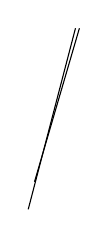
\begin{tikzpicture}\draw (0,0)--(.6,2.3);\draw (.08,.35)--(.65,2.3);\end{tikzpicture}}
\margin{Cette compatibilité peut déjà \unsure{s'énoncer} pour analytique $\longleftrightarrow$ \unsure{topologique} (\unsure{avec classes de corr. analytiques})}

\margin{Ouf !}
\mspage{24}

\scanpage{26}
SYSTÈMES de RACINES (12) \hfill Tribu n° 59

§ 9. \uuline{Classification des \unsure{6tèmes} de racines.}

\uline{n° 1} - Dire qu'on est sur $R$, (l.2 du n° 1). A la l.5 bas de la p. 177 remplacer ``Il s'agit'' par ``Nous allons''. En bas de la p. 177, indexer par un ensemble $I$ à $\ell$ éléments, ce qui simplifie. Remonter la prop. 1 à la p. 178, (les murs étant indexés par $I$ et $I'$). Dessiner qq. chose dans le trou de la p. 178.

Il est antibourbachique que les lemmes aient des corollaires : les corollaires des pp. 179 sqq. seront qualifiés de lemmes. Dans le lemme 1, considérer l'ensemble $J$ des $j$ liés à $i$. Mieux expliciter le procédé d'identification de la p. 180 : on part d'une arête $(i,j)$ d'ordre 3 ; on enlève $i$, $j$ de l'ensemble des sommets, et on y met un nouveau sommet $p$ ; les arêtes sont, d'une part les anciennes ne contenant ni $i$ ni $j$, d'autre part, si $(i,k)$ ou $(j,k)$ est une vieille arête, $(p,k)$ sera une nouvelle arête ; les ordres sont conservés ; algébriquement, ça revient à remplacer les variables $\xi_i$ et $\xi_j$ par une nouvelle variable $\xi_p$.

Enoncé du haut de la p. 181, (devenu lemme) : ou bien un seul point de ramif. et toutes arêtes d'ordre 3, ou bien chaîne et au plus une arête d'ordre $\geq4$.

Les lemmes 3 et 4 ont l'air, soit canulés, soit d'énoncés tirés par les cheveux ; revenir à l'état 3, (n° 383), où c'était plus clair.

La prop. 1 remonte au début du n°.

\uline{n° 2} - Commencer par : nous allons voir que ces trois zèbres correspondent à des groupes ; y peuvent pas provenir de systèmes de racines à cause des 5 ou des $p\geq7$, (référence) ; par contre, nous verrons plus loin que tous les autres proviennent de systèmes de racines. A la fin du n°, dire que les formes obtenues

\mspage{25}

\scanpage{27}
Soit $K$ un corps top. isomorphe à $\mathbf C$ [isom non choisi !]

Alors on a le foncteur \inserted{\unsure{mult.}} $\xi=\xi_K$ sur la catégorie des motifs sur $K$, à valeurs dans les $\mathbf Z$-modules, et des isom
\[
 \xi\otimes_{\mathbf Z}\mathbf Z_\ell\overset{\alpha_\ell}{\simeq}\unsure{\xi}_\ell
\]
\[
 \xi\otimes_{\mathbf Z}K\overset{\alpha_\infty}{\simeq}\xi_K
\]
Considérons
\[
 \xi\bigl(H^2(\mathbf P^1,\unsure{\mathbf Z}(\infty))\bigr)=\xi(\mathbf Z(-1))
\]
c'est isomorphe à $\mathbf Z$, l'isom n'étant pas choisi. Le choix d'un tel isom \inserted{``\unsure{au dire des géom.}''} revient à celui d'une \uline{orientation} sur $\mathbf P_K^1$ [qui est de façon naturelle une variété \deleted{algébrique} réelle, isomorphe à $S^2$), ou ce qui revient au $\unsure{=}$, au choix de l'une des deux structures complexes sur $\mathbf P_K^1$, provenant du \inserted{choix d'un} isom $K\simeq\mathbf C$, i.e. le choix d'\uline{une} des racines de $-1$ dans $K$. Comme $\pi\in\mathbf R\subset K$ est bien déterminé comme

\mspage{26}

\scanpage{28}
SYSTÈMES de RACINES (5) \hfill Tribu n° 59

racine simple $v_i$ envoie $v_i$ en $-v_i$ et permute les autres racines positives. Donner un lemme sur les applic. $R\longrightarrow\text{groupes}$.

Les n° 6 et 7 sont permutés.

\uline{n° 6} - (Ensembles clos de racines ; ancien n° 7).

Ajouter la prop. 4 de Serre, (n° 400, Annexe II), et sa prop. 5 ; par contre, son cor. et le lemme 2, (p. A.11), passent en exer.

Pour la prop. 15, on prend la démonstration suivante, (fournie par Borel) :

\uline{p. 110}. \uline{Prop. 15}. Démonstration :

1) Remarquons d'abord que si $x=a.y$, $(x,y\in P)$, alors $a>0$. Sinon, en effet comme $a\ne-1$ vu l'hypothèse $P\cap-P=\varnothing$ on peut, en changeant éventuellement les rôles de $x$ et $y$, supposer $a=-1/2$, d'où $x+y=y/2\in P$ et $y/2$, $-y/2\in P$, ce qui est absurde. Il s'ensuit, compte tenu de la Prop. 4 du N° 3 que si $x$, $y\in P$ et $(x,y)<0$, alors $x+y\in P$.

2) Montrons maintenant qu'aucune somme $y_1+\ldots+y_q$, $(q\geq1)$, d'éléments de $P$ n'est nulle. On procède par récurrence sur $q$ ; le cas $q=2$ résultant de $P\cap(-P)=\varnothing$, on peut supposer $q\geq3$. Si $y_1+y_q=0$, alors $-y_1=y_2+\ldots+y_q$ donc $(-y_1,y_2+\ldots+y_q)>0$, d'où l'existence d'un indice $j$ $(1\leq j\leq q)$ tel que $(y_1,y_j)<0$. On a alors $y_1+y_j\in P$ et :
\[
 (y_1+y_j)+\sum_{1\leq i\leq q,\,i\ne j}y_{\unsure{1|i}}=0,
\]
contrairement à l'hypothèse de récurrence.

3) Nous voulons montrer maintenant l'existence d'un élément $z\ne0$ de $V$ tel que $(z,x)\geq0$ quel que soit $x\in P$. Si ce n'est pas le cas, alors, vu (1), on

\mspage{27}

\scanpage{29}
élément de $K$, on voit que le choix ainsi fait permet d'écrire
\[
 \alpha_\infty(u)=\frac{1}{2\sqrt{-1}\pi}\,v
\]
où $v$ est le générateur canonique de $H^1(\mathbf P^1,\Omega^1)$.

Pour les choix différents de topologie sur $K$ faisant de $K$ un corps valué complet arch., on trouve ainsi tous les éléments \unsure{primitifs|possibles} de $H^1(\mathbf P^1,\Omega^1)$.

Si $K$ est un corps \deleted{\unsure{top.}} isom à $\mathbf R$ [l'isom étant d'ailleurs \uline{unique}], alors on définit encore, par choix de $\mathbf C$ comme \deleted{\unsure{complexe}} clôture algébrique de $\mathbf R$, un foncteur $\xi=\xi_K$ à valeurs dans les modules sur $\mathbf Z$, \deleted{et \unsure{des isom}} \inserted{mais avec op. de $\mathbf Z/2\mathbf Z=\operatorname{Gal}(\overline{\mathbf R}/\mathbf R)$}. Le sous \unsure{$\mathbf Z$|$\mathbf Q$}-réseau \inserted{$\xi(M)$} que nous obtenons dans $\displaystyle\prod_\ell M_\ell\times M_{\infty\mathbf C}$ \inserted{\unsure{relatif :} $\mathbf R\hookrightarrow\mathbf C$} est alors stable par ce groupe $\mathbf Z/2\mathbf Z$

\mspage{28}

\scanpage{30}
\mspage{29}
SYSTÈMES de RACINES (10) \hfill Tribu n° 59

un quotient sur un anneau $A$ qqconque ; ce quotient est unique car $d$ n'est pas diviseur de zéro. Pour (ii), on écrit $d=\sum_x c_x Qe^x$, (cf. prop. 7) ; or, dans $d$, il y a un terme en $e^{w_0}$, et tous les autres sont plus petits, (pour l'ordre défini par $P^+$) ; comme les $x$ sont $\geq w_0$, il y a un seul terme dans la somme, avec coeff. 1.

Le haut de la p. 162, (3 lignes), aura déjà été dit.

§ 8. \uuline{Transformations de Coq-se-taire.}

\uline{n° 1} - Le lemme 6 du § 6, n° 13 remonte ici.

\uline{n° 2} - Dans le 2) en bas de la p. 163, prendre seulement $g=s_1$. Dans le lemme 1, on notera $L$ le monoïde, $Y$ l'ensemble des $n!$ mots et $C(X)$ le graphe. Dans l'énoncé, remplacer 2) par : `` y'a un mot $A$ et un sommet $b$ tels que $u=Ab$ et $v=bA$ '' ; ça simplifie la démonstration. Mieux expliquer comment la connexion du graphe donne la conjugaison voulue.

La fin de la démonstration, (p. 165), se simplifie ainsi : il y a deux cas ; si $a$ et $b$ sont non liés, c'est facile comme dans le texte ; si $a$ et $b$ sont liés, alors $a$ n'est lié à aucun élément de $A$, et on passe de $bAa$ à $Aba$ par les étapes $bAa$, $baA$, $aAb$, $Aba$.

\uline{n° 3} - Commencer par un laïus introduisant les $m_i$, (avec déf. en forme des exposants), et donnant les formules (1), (2), (3), (numérotées), qui sont des trivialités. Puis une proposition, réduite à (ii) et (iii), où on supposera $G$ irréductible, ((ii) est faux avec $G$ réductible). Pour la démonstration, on

\scanpage{31}
Corps de \unsure{base} top. $\simeq\mathbf R$ ou $\mathbf C$

(foncteurs de Hodge et \unsure{De Rham} dans ce cas)

\mspage{30}

\scanpage{32}
INSTITUT\\
DES HAUTES ÉTUDES SCIENTIFIQUES\\
BURES-SUR-YVETTE (S.-\&-O.)\\
928-48-53

\uline{Corps de base topologique isom. \unsure{à} $\mathbf R$ ou $\mathbf C$}

$K$ corps topologique isom. \unsure{à} $\mathbf C$ (il y a donc \uline{deux} isom avec $\mathbf C$, mais on ne choisit pas). $K$ contient can. $\mathbf R$.

$M$ motif sur $K$. Alors \deleted{$\operatorname{DR}(M)$ \unsure{De Rham}} pour \unsure{tt} $X$ lisse projectif sur $K$, $X(K)$ est un espace topologique cpt (variété $K$-analytique compacte), d'où $H^*(X,\mathbf Q)$, et on définit ainsi \uline{foncteur de Betti} $M\rightsquigarrow\operatorname{Betti}(M)$ sur les motifs sur $K$. $\operatorname{Betti}(M)\otimes_{\mathbf Q}K$ $\unsure{\simeq}$ canoniquement à $H^*(X,K)$. Par l'argument habituel, ce dernier est isomorphe can. à la coh. de De R., d'où
\[
\operatorname{Betti}(M)_K\simeq\operatorname{DR}(M)
\qquad\otimes\text{-isom can.}
\]
Ceci met sur \inserted{(ce $K$-vecteur)} $\operatorname{DR}(M)$ une structure \uline{réelle}, dont le sous-espace réel est $\operatorname{Betti}(M)_{\mathbf R}$ ; soit $\sigma$ l'involution. La filtration canonique de $\operatorname{DR}(M)$, et $\sigma$, permettent de façon unique de splitter cette filtration, de façon à obtenir sur $\operatorname{DR}(M)$ une \uline{bigraduation} compatible avec les degrés \unsure{totaux}, et \unsure{redonnant} la filtration can. à l'aide du premier degré. Le choix d'un isom $\unsure{\pi|i}:K\unsure{-|\longrightarrow}\mathbf C$ met, par transport de str., une

\mspage{31}

\scanpage{33}
structure \inserted{de vecteur} complexe sur $\operatorname{DR}(M)$ ; mais on voit que la bigraduation déduite par transport de structure de celle de Hodge ne \uline{dépend pas de $\pi$} (donc, si on remplace $\pi(\lambda)$ par $\overline{\pi(\lambda)}$, elle n'est \uline{pas} remplacée par la symétrique !).

\inserted{Néanmoins, si on regarde, pour un motif donné $M$, le motif $\unsure{{}^{c}M_{\underline c}}$ ($\underline c$ l'aut. non trivial de $K$) sur $\operatorname{DR}({}^{c}M_{\underline c})\xrightarrow{\sim}\operatorname{DR}(M)_{\underline c}$, les structures \unsure{rationnelles}, \inserted{(et filtrations)} et les $\unsure{\sigma}$, \unsure{Ainsi|Alors} \deleted{la filtration} composant avec $\sigma$, on trouve un \uline{$K$-isom} $\operatorname{DR}(M_{\underline c})\simeq\operatorname{DR}(M)$, conservant la $\mathbf Q$-structure, et \uuline{renversant} \inserted{les} \unsure{filtrations}.}

\deleted{\unsure{Supp.}} Soit maintenant $K_0=\mathbf R$, et considérons motifs \inserted{$M$} \uline{sur} $\mathbf R$. Choisissons une clôture alg. $K$ de $K_0=\mathbf R$. Alors $\operatorname{DR}(M)_K=\operatorname{DR}(M_K)$ est muni de \uline{deux façons} d'une $\mathbf R$-structure : du fait qu'il est déduit de $\operatorname{DR}(M)$ par $\mathbf R\unsure{-|\longrightarrow}K$, et puis : la construction donnée plus haut. Soit $\sigma$ l'autom de conjugaison complexe défini plus haut, (N.B. $\sigma$ \uline{ne respecte pas} la \uline{filtration}) $\tau$ celle définie par $\operatorname{DR}(M)_K\simeq\operatorname{DR}(M_K)$ (donc $\unsure{\sigma|\tau}$ respecte la filtration) - $\sigma$ et $\tau$ sont \uline{semilinéaires}. Alors $\sigma$ et $\tau$ commutent, en d'autres termes $\operatorname{DR}(M_K)^\sigma$ $(\simeq H^*(X(K),\mathbf R)$ si $M=\operatorname{Mot}^*(X))$ est stable par $\tau$ : en effet, $\tau$ n'est autre que l'autom de $H^*(X(K),\mathbf R)$ défini par l'autom $\tau_X$ de $X(K)$ ! Alors $\sigma\tau=\tau\sigma=\unsure{f_{\mathbf R}|\mathfrak f_{\mathbf R}}$ est l'autom de $H^*(X(K),K)\simeq\operatorname{DR}(\operatorname{Mot}^*(X))$

\margin{$X(K)$}
\mspage{32}

\scanpage{34}
défini par l'aut \deleted{\unsure{de}} $\tau_X$ de $X(K)$. Ainsi, un motif sur $\mathbf R$ définit :

a) Une structure de Hodge $V$ sur $K$

b) Un autom $f_{\mathbf R}$ \inserted{de carré 1} du $K$-espace vectoriel \deleted{sousjacent} \inserted{$V_K$}, cet autom étant ``réel'' i.e. qui transforme $V_{\mathbf R}$ dans $V_{\mathbf R}$, et $\mathbf Q$-\uline{rationnel} i.e. transforme $V$ en $V$

\deleted{\unsure{La réciproque|La conjugaison}}

Ces deux données étant assujetties à la condition
\[
\left\{\begin{array}{l}
(f_{\mathbf R})\sigma\ \text{\unsure{invarie} la filtration naturelle}\\
\text{i.e. }f_{\mathbf R}\ \text{échange la filtration donnée et l'opposée}
\end{array}\right.
\]
En termes de ``\unsure{donnée de descente}'', on peut \deleted{\unsure{dire aussi}} \inserted{exprimer} aussi b) en disant qu'on a un isom de la structure de Hodge $V$ avec la structure de Hodge \deleted{\unsure{qui}} ``conjuguée'' : c'est le frobenius réel.

Soit $G$ le groupe de Galois motivique de $M$ sur $\mathbf R$. Alors $f_{\mathbf R}$ correspond à un élément
\[
f_{\mathbf R}\in G(\mathbf Q)
\]
appelé \uline{frobenius réel}. C'est un élément d'ordre 2. Son image dans $G/G^0$ engendre ce groupe. Cet élément normalise $\underline i:S_{\mathbf R}\longrightarrow G_{\mathbf R}$, de façon précise
\[
f_{\mathbf R}i(\lambda)f_{\mathbf R}^{-1}=i(\deleted{\unsure{\lambda}}\lambda')
\qquad\text{où }\lambda\mapsto\lambda'\text{ est la symétrie canonique de }S_{\mathbf R}.
\]
Donc sur $U_{\mathbf R}$ on a
\[
(*)\qquad f_{\mathbf R}i(\lambda)f_{\mathbf R}^{-1}=i(\lambda^{-1})
\qquad (\lambda\in U_{\mathbf R}\deleted{\unsure{(\mathbf R)}})
\]
Le foncteur $M\mapsto(\text{structure de Hodge associée, avec }f_{\mathbf R})$ est pleinement fidèle en vertu des conj. de Hodge.

\margin{\unsure{Les structures en jeu sont donc} $G$ sur $\mathbf Q$, $\varepsilon:G\to G_m$, $i:S_{\mathbf R}\unsure{-|\longrightarrow}G_{\mathbf R}$ (avec $i\vert G_{m\mathbf R}$ défini sur $\mathbf Q$ etc) $+f_{\mathbf R}\in G(\mathbf Q)$, satisfaisant les conditions \unsure{exp.}}
\mspage{33}

\scanpage{35}
INSTITUT\\
DES HAUTES ÉTUDES SCIENTIFIQUES\\
BURES-SUR-YVETTE (S.-\&-O.)\\
928-48-53

Les éléments de $\operatorname{DR}(M)$ sont les éléments de $\operatorname{DR}(M)_K\simeq V\otimes_{\mathbf Q}K$ de la forme $z=x+iy$ $(x,y\in V_{\mathbf R})$ avec $x=fx$, $y=-fy$ (on exprime $\tau z=z$ i.e. $f\sigma z=z$ i.e. $\sigma z=fz$).

\deleted{\unsure{Ceci|C’est à}} Donc l'espace $\operatorname{DR}(M)$ admet une \inserted{$\mathbf Q$-structure de} façon naturelle \deleted{\unsure{de structure}} : on prend le sous-espace des $x+iy$, $x,y\in V$, $x=fx$, $y=-fy$. Soit $W$ cet espace, il mérite le nom de \uline{sous-espace de Betti} \inserted{\uline{tordu}} de $\operatorname{DR}(M)$.

Il est stable par $f$. Mais la formation de ce sous-espace \unsure{se comporte-t-il} comme il faut par $\otimes$ ? \uline{Oui}.

\diagram{\begin{tikzcd}[ampersand replacement=\&,column sep=small,row sep=large]
H^{\unsure{*|0}}(X(K),\mathbf Q)=V
 \arrow[r,phantom,"\subset" description]
 \arrow[d,phantom,"\cup" description]
\& \operatorname{DR}(M)_K\simeq\operatorname{DR}(M_K)
 \arrow[d,phantom,"\cup" description]\\
H^{\unsure{*|0}}(X(\mathbf R),\mathbf Q)=V\cap W=V^f=W^{\unsure{F|f}}
 \arrow[r,phantom,"\subset" description]
\& W
\end{tikzcd}}

On a ainsi un deuxième foncteur fibre sur $\mathcal M$ à valeurs dans $\mathbf Q$, mais il est isom \inserted{comme foncteur \unsure{$\oplus$-isant|$\otimes$-isant}} au premier, \deleted{\unsure{en effet}} comme on voit en écrivant $V\simeq V^++V^-$, $W=W^++W^-$, et utilisant les isomorphismes $V^+\simeq W^+$, $V^-\simeq W^-$ canoniques. Cet isom $V\unsure{-|\longrightarrow}W$ est \inserted{\unsure{$f$.}} induit par l'autom de $\operatorname{DR}(M_K)\simeq V_K\simeq W_K$ qui est l'identité sur $V_K^+$, et la multiplication par $i$ sur $V_K^-$ ; Cependant, cet isom \uline{n'est} \uline{pas} compatible avec le produit \uline{tensoriel}.

Il semble que $\operatorname{Betti}^T$ et $\operatorname{Betti}$ ne sont \unsure{pas $\otimes$ isom}, l'un est déduit de l'autre en tordant par le cocycle défini par $f_{\mathbf R}$ ----
\margin{Betti tordu}
\mspage{34}

\scanpage{36}
L'élément $\alpha\in P(\mathbf C)$ est relié à $f_\infty$ par
\[
\overline\alpha=f_\infty\alpha
\]
donc $f_\infty$ à priori
\[
\left(f_\infty=1\Longleftrightarrow\alpha\in P(\mathbf R)\quad\text{i.e.}\quad\mathbf R(\alpha)=\mathbf R\right)
\]
\deleted{Comme on a la relation $f_\infty\unsure{j_1}f_\infty=\unsure{j_2}$, cette condition implique $j_1=j_2$ donc $j_1=j_2=\frac12 i$, i.e. \deleted{$\unsure{G}$} [si on admet conj. de Hodge] $G^0\xrightarrow[\sim]{\varepsilon}G_m$}

Or on vérifie aussitôt
\[
\boxed{\varepsilon(f_\infty)=-1}
\]
ce qui nous montre qu'on a \unsure{tjrs}
\[
\boxed{f_\infty\ne1\quad\text{i.e.}\quad\mathbf R(\alpha)=\mathbf C}
\qquad\text{(si $M$ contient le motif de Tate)}
\]
Si $M$ ne contient pas le motif de Tate, on voit que $f_\infty=1\Longrightarrow j_1=j_2$ i.e. $j_1=j_2=\frac12 i$, donc en vertu de la conj. de Hodge, il faut que $G^0=\operatorname{Im}\unsure{j_2|j_1}$, donc ou bien $G^0=\{e\}$ \deleted{(motifs de dimension 0, sur $G=\{e\}$ \unsure{ou} $\mathbf Z/2\mathbf Z$, dans ce dernier cas $f_\infty$} \inserted{ici $G=G^0$ car $\unsure{f_\infty}$} \inserted{donc $G=1$} [\uline{NB} si $G$ est disconnecté, on sait que $f_\infty\notin G^0(\mathbf Q)$], ou bien $G=G_m/\mu_n$, $n\geq1$, $M$ est \deleted{\unsure{produit de}} engendré par $\mathbf Q(-n)$\} ; on trouve en $\unsure{=}$ temps que $n$ est \uline{pair}. Donc on trouve

\diagram{\begin{tikzcd}[ampersand replacement=\&,column sep=large,row sep=large]
(f_\infty=1)\arrow[r,Leftrightarrow]
\& (\mathbf R(\alpha)=\mathbf R)\arrow[r,Leftrightarrow]
\& \begin{array}{c}M\text{ est engendré par }\mathbf Q(-2n),\\\text{un quelconque }n\geq0.\end{array}\arrow[d,Leftrightarrow]\\
\&\&G\simeq G_m\text{ ou }G\simeq\{e\}
\end{tikzcd}}
\margin{moyennant conj. de Hodge}

\margin{\fbox{\parbox{0.88\linewidth}{\uline{NB} $f_\infty$ ne peut être \uline{\unsure{central}} que si $G^0=\operatorname{Im}\deleted{\unsure{j}}i$, ce qui implique que $M$ est \deleted{engendré} contenu dans la cat. engendrée par $\mathbf Q$ \unsure{tordu} et par $\mathbf Q(2)$. Il revient au $\unsure{=}$ dire que $G$ est \uline{\unsure{comm.}}}}}
\mspage{35}

\scanpage{37}
\uline{Motifs sur $\mathbf R$}

$\mathcal M$ \inserted{$\otimes$} catégorie de motifs sur $\mathbf R$, $G=\underline{\operatorname{Aut}}_\otimes(T_B)$ groupe de Galois associé.

Notons qu'on a un $\otimes$-automorphisme d'ordre 2 de $T_B$, qui sur la catégorie $\mathcal V_{\mathbf R}$ des var. proj. lisses $X$ sur $\mathbf R$ revient à l'automorphisme des $H^*(X(\mathbf C),\mathbf Q)$ défini par l'autom $x\mapsto\bar x$ de $X(\mathbf C)$. D'où
\[
\boxed{f_{\deleted{\mathbf R}\infty}\in G(\mathbf Q)}
\qquad(f_{\unsure{\infty|\mathbf R}}^2=1),
\]
(``frobénius réel''). \deleted{On retrouve le sous-espace $H^*_{\mathrm{DR}}(X)$ de $H^*(\unsure{X|X(\mathbf C)},\unsure{\mathbf C|\mathbf Q})=+$} Si $\sigma_M$ est la conjugaison complexe de $M\otimes_{\mathbf Q}\mathbf C$ [où $M\in\operatorname{Ob}\operatorname{Rep}(\unsure{C|G})$], alors la conjugaison $\tau_M$ associée à la structure réelle $T_{\mathrm{DR}}(M)\subset M\otimes_{\mathbf Q}\mathbf C$ n'est autre que
\[
\tau_M=(f_{\unsure{\infty|\mathbf R}})_M\sigma_M
=\sigma_M(f_{\unsure{\infty|\mathbf R}})_M
\]
Donc on retrouve grâce à $f_\infty$ la structure \unsure{mixte|réelle} sur les $M\otimes_{\mathbf R}\mathbf C$, donc aussi le torseur
\[
P=\underline{\operatorname{Isom}}_\otimes(T_B\otimes_{\mathbf Q}\mathbf R,T_{\mathrm{DR}})
\]
sur $G_{\mathbf R}$ : c'est celui défini par le 1-cocycle \deleted{de} \unsure{non abélien} sur $\Gamma=\mathbf Z/2\mathbf Z$, à coeff dans $G(\mathbf C)$, dont la valeur en l'élément $\ne e$ est $f_\infty$. La forme tordue correspondante de $G$ s'obtient en prenant sur $G_{\mathbf C}$ la donnée de descente associée à \deleted{$\unsure{f}$} $\operatorname{int}(f_\infty)\times_{\mathbf R}\sigma_{\mathbf C}$. \deleted{On sait donc, pour} La relation entre $f_\infty$ et
\[
j:S_{\mathbf R}\longrightarrow G_{\mathbf R}
\]
est que
\[
\boxed{f_\infty j(\lambda)f_\infty^{-1}=j(\unsure{\lambda'|\bar\lambda})},
\]
où $\lambda\mapsto\lambda'$ est l'autom can. de $S_{\mathbf R}$ (donnant $\lambda\mapsto\bar\lambda$ sur $S_{\mathbf R}(\mathbf R)\simeq\mathbf C^*$)
\mspage{36}

\scanpage{38}
D'autre part, on aura ici
\[
\beta\in Q(\mathbf R)\subset P'(\mathbf R)
\]
donc
\[
\mathbf R(\unsure{\gamma|\sigma})=\mathbf R(\beta,\gamma)=\mathbf R(\beta,\alpha)=\mathbf R(\alpha)
\]
et par suite
\[
\mathbf R(\unsure{\gamma|\sigma})=\mathbf R(\alpha)
\]
qui est donc $=\mathbf C$ sauf dans le cas exceptionnel précisé plus haut.

\uline{Remarque} Soit $M$ un motif sur $\mathbf R$, correspondant à un \deleted{$G$-module} \deleted{\unsure{associé}} $T_B(M)$. Alors on ne peut avoir $f_{\infty M}=\operatorname{id}_M$ que si $M$ est une somme de puissances tensorielles de $\mathbf Q(2)$.

\figure{\begin{tikzpicture}\draw (0,0)--(.8,.03);\end{tikzpicture}}

\deleted{La relation
\[
f_\infty j(\lambda)f_\infty^{-1}=j(\lambda')
\]
implique, faisant $\lambda=C\in S(\mathbf R)$
\[
f_\infty C f_\infty^{-1}=C^{-1}=\eta C\qquad(\eta=i(-1))
\]
donc
\[
f_\infty\in\underline{\operatorname{Norm}}_{G_{\mathbf R}}(C,C^{-1})
\]
\deleted{Or, \unsure{comme} $K'=\underline{\operatorname{Norm}}_{G_{\mathbf R}}(C,C^{-1})\supset\underline{\operatorname{Norm}}_{G_{\mathbf R}}(C)=K$ qui est un sous-groupe d'indice 1 ou 2. On sait que $K(\mathbf R)$ est un compact maximal dans $G(\mathbf R)$} Considérons $G/i(G_m)=\dot G$ $[=\operatorname{Ker}\varepsilon/\underline i(\mu_2)]$, et les images $\dot f_\infty$, $\dot C$ de $f_\infty$, $C$, donc on a
\[
\dot f_\infty\in\underline{\operatorname{Norm}}_{\dot G_{\mathbf R}}(\dot C,\dot C^{-1})\overset{\mathrm{dfn}}=K'
\]
Or \deleted{on sait que} \unsure{soit}
\[
K=\underline{\operatorname{Norm}}_{\dot G_{\mathbf R}}(\dot C)\subset K'
\]
}
\mspage{37}

\scanpage{39}
\deleted{\unsure{Soit}}

Soit $K$ un corps topologique isomorphe à $\mathbf C$, $X$ un schéma algébrique défini sur $K$. Alors $X_{\mathrm{top}}$ est défini, et aussi $H^*(X_{\mathrm{top}},K)$. D'autre part, \inserted{si $X$ est non sing.,} la cohomologie de Hodge est définie, \unsure{soit} $H^*(X)$ [indépendant de la structure topologique de $K$]. Alors le choix d'un isom top. $u:K\unsure{-|\longrightarrow}\mathbf C$ définit un isomorphisme
\[
H^*(X_{\mathrm{top}},K)\xrightarrow{\sim}H^*(X)
\]
et on vérifie aussitôt que cet isomorphisme ne dépend pas du choix de $u$. [En d'autres termes, si $K=\mathbf C$, alors les deux homomorphismes
\diagram{\begin{tikzcd}[ampersand replacement=\&,column sep=large,row sep=large]
\& H^*(X)\arrow[dd,"{\text{(antilinéaire)}}"]\\
H^*(X_{\mathrm{top}},\mathbf C)\arrow[ur]\arrow[dr]\arrow[phantom,r,"{\text{non comm.}}"{description,xshift=-6pt}]
 \& {}\\
\& H^*(X^c)
\end{tikzcd}}
(où $c:\mathbf C\unsure{-|\longrightarrow}\mathbf C$ est la conjugaison complexe) sont \deleted{conjugués} déduits l'un de l'autre par application de $c$ aux coefficients dans $H^*(X_{\mathrm{top}},\mathbf C)$]

\inserted{Cela nous permet, notant qu'on a un \unsure{isom injectif|hom injectif} continu unique $u:\mathbf R\to\mathbf C$, de définir $H^*(X_{\mathrm{top}},\mathbf R)\hookrightarrow H^*(X)$ (même si $X$ pas définissable sur $\mathbf R$ !) d'où une sous-\inserted{$\mathbf R$-}algèbre de $H^*(X)$, \deleted{\unsure{définie sur $\mathbf R$}} notée $H^*(\unsure{X_{\mathrm{top}}|X},\mathbf R)$ \deleted{$H^*(X)^{\unsure{+}}$} \deleted{\unsure{cela indépendant de la topologie de $K$}}, on obtient $H^*(X)^-=\sqrt{-1}H^*(X)^+$}

\figure{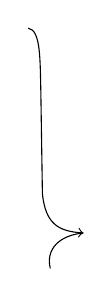
\begin{tikzpicture}[x=1cm,y=1cm]
\draw[->] (0,2.7) .. controls (.16,2.68) and (.15,2.3) .. (.16,1.9) -- (.18,.6) .. controls (.22,.2) and (.4,.12) .. (.7,.1);
\draw (.28,-.35) .. controls (.22,-.1) and (.4,.07) .. (.7,.1);
\end{tikzpicture}}

Supposons $X$ projective non \uline{singulière}, alors le choix d'un isom top. $u:K\xrightarrow{\sim}\mathbf C$ définit une décomposition
\[
\varphi:\coprod_{p,q}H^q(X,\Omega_X^p)\xrightarrow{\sim}H^*(X)
\]
compatible avec la filtration de $H^*(X)$. On vérifie encore que $\varphi$ est indépendant du choix de $u$.
\mspage{38}

\scanpage{40}
Enfin, supposons maintenant que $K$ soit isomorphe $\mathbf R$ [on peut supposer $K=\mathbf R$, car $\mathbf R$ n'a pas d'autom. non trivial] soit $K'$ une clôture algébrique de $K$, $\pi=\mathbf Z/2\mathbf Z$ son groupe de Galois, $X$ lisse \deleted{\unsure{propre}} [projectif] sur $K$. Alors on peut appliquer ce qui précède à $X_{K'}$ sur $K'$. On trouve
\deleted{\[
 H^*(X_{\unsure{K'\mathrm{top}}},\mathbf R)\unsure{\xrightarrow{\sim}}H^*(X)\otimes_K K',
\]}
\[
 [\varphi_{K'}:\coprod_{p,q}H^q(X,\Omega_X^p)\otimes_K K'
 \xrightarrow{\sim}H^*(X_{\deleted{\unsure{K}}})\otimes_K K']
\]
et d'après ce qui a été vu plus haut, cet isomorphisme \uline{commute à} $\pi$, donc provient d'un isomorphisme
\[
 \varphi_{\unsure{i|K}}:\coprod_{p,q}H^q(X,\Omega_X^p)\xrightarrow{\sim}H^*(X).
\]

\margin{On a aussi un $\mathbf R$-isom canonique $(\pi=\mathbf Z/2\mathbf Z)$
\[
 H^*(X_{\mathbf C\mathrm{top}},\mathbf R)\otimes_{\mathbf R}\mathbf C
 \xrightarrow{\sim}H^*(X)\otimes_{\mathbf R}\mathbf C,
\]
où $\pi$ opère : à gauche via son opération sur $X_{\mathbf C\mathrm{top}}$ \uline{et} sur $\mathbf C$ dans $\otimes_{\mathbf R}\mathbf C$
d'où en passant aux invariants sous $\pi$ une décompos. canonique
\[
 H^*(X)\simeq H^*(X)^+\oplus H^*(X)^-,\qquad
 H^*(X)^+\simeq H^*(X_{\mathbf C\mathrm{top}},\mathbf R)^\pi
 =H^*(X_{\mathrm{top}}=X_{\mathbf C\mathrm{top}}/\pi;\mathbf R),
\]
\deleted{$H^{\unsure{*}}(\unsure{X},\mathbf R)$}
\[
 H^*(X)^-=H^*(X_{\mathbf C\mathrm{top}},\unsure{\mathbf R})^-.
\]}

En résumé, chaque fois que $X$ est projectif non singulier sur un corps \deleted{\unsure{top.}} top. loc. cpt complet archimédien, on a une décomposition $\varphi$ en une somme de $H^*(X)$, compatible avec la filtration. \deleted{Si} On pose
\[
 \boxed{H^{p,q}(X)=\varphi(H^q(X,\Omega_X^p))\subset F^pH^q(X)}
\]
Si $K$ n'est pas topologique, alors pour tout choix d'une topologie \unsure{formée|fermée} archimédienne $T$ sur $K$, on obtient sur
\mspage{39}

\scanpage{41}
\[
 H^*(X)_T=H^*(X)\otimes_K\widehat K_T.
\]
une décomposition
\[
 \boxed{\varphi_T:\coprod_{p,q}H^q(X,\Omega_X^p)_T\longrightarrow H^*(X)_T}
\]
Cela permet de définir
\[
 H_T^{p,q}(X)=\varphi_T(H^q(X,\Omega_X^p)_T)\cap H^*(X)\subset F^p(H^q(X))
\]
qui est un \uline{sous-\inserted{$K$-}espace vectoriel de} $H^*(X)$, défini canoniquement par la donnée de $T$. Nous poserons de \unsure{$=$}
\[
 H_T^{pq}(X,\mathbf R)=\varphi_T(H^q(X,\Omega_X^p)_T)\cap H^*(X_{\unsure{\widehat K_T}},\mathbf R)\cap H^*(X)
\]
\deleted{c'est un \unsure{sous-} \deleted{$\unsure{K}$} $\unsure{\mathbf R,K}$-espace vectoriel de}
c'est encore un sous-\inserted{$K$-}espace vectoriel de $H^*(X)$ si $\widehat K_T\simeq\mathbf R$; \deleted{sinon} \inserted{$\widehat K_T\simeq\mathbf C$} c'est un sous-\deleted{$\unsure{R_{\mathrm{top}}}$}$R_T$-espace vectoriel, où
\[
 R_T=\mathbf R\cap K,\qquad\text{dans }\widehat K_T\simeq\mathbf C
\]
[sous-\uline{corps réel} pour $T$]; à fortiori, \deleted{\unsure{est}} dans tous les cas, on obtient un $K_r$-espace vectoriel, où
\[
 K_r\simeq\bigcap_T R_T\simeq\text{plus gd sous-corps tot. réel de }K
\]
(NB $K_r$ est une ext. algébrique du corps premier $\mathbf Q$).
\mspage{40}

\scanpage{42}
Variation du réseau discret en \unsure{termes|terme} d'une place archimédienne,

Critère de transcendance
\mspage{41}

\scanpage{43}
\uline{Pbs}

\deleted{\uline{\unsure{Pbs}}}

\diagram{\[
\begin{array}{ll}
\text{1) Betti, De-Rham}&
\left\{\begin{array}{ll}
a)&\text{Comparaison ``réseaux'' de De Rham et \deleted{\unsure{avec}} de Betti}\\
b)&\text{Comparaison réseaux de Betti \uline{pour topologies différentes!}}\\
c)&\text{Comparaison structures réelles, \uline{resp. splittages}, (dans De Rham)}
\end{array}\right.
\end{array}
\]}

2) Betti, $\ell$-adique\qquad \deleted{\unsure{Comp.}} Comparaison de réseaux de Betti pour top. diff.
(dans ch. \uline{$\ell$-adique})

3) DeRham, $p$-adique\qquad Sur un corps valué \inserted{(complet \unsure{discrètem.})} (non archimédien), \inserted{corps résiduel car $p$]} comparaison possible entre cohomologie $p$-adique et cohomologie de DeRham ?

4) Définition de cohomologie $p$-adique en car $p>0$ ?
\mspage{42}

\scanpage{44}
\begin{flushright}32\end{flushright}

the induction assumption that the right hand side is a polynomial in $n$, of degree not higher than $s-1$. Therefore, $X(V^*,K_n^*)$ is a polynomial in $n$, of degree not higher than $s$.

The line from above will mean that we have a direct image, corresponding to the mapping $f$. There occurs an imbedding $K\to\bar K'$ [See (${}^8$)]. To the imbedding $O'_V\to O_{V^*}$ corresponds the homomorphism
\[
 K'\otimes_{O'_V}O'_V\longrightarrow K'\otimes_{O'_V}O_{V^*}
\]
or, what comes to the same thing, $K'\to K^*$.

Turning to the direct images, we obtain the homomorphism $\bar K\to\bar K^*$ and hence the homomorphism $\bar K\to\bar K\unsure{*|{}_*}$.

Let $W$ be the variety of singularities of the variety $V$,
\[
 U_W=V-W,\qquad U'_W=f^{-1}(U_W).
\]
$f$ establishes biregular correspondence between $U_W$ and $U'_W$.

\margin{p. 192}
Evidently, the homomorphisms $K|U_W\to\bar K'|U_W$ and $O'_V|_{U'_W}\to O_{V^*}|_{U'_W}$ are isomorphisms. Hence it follows that $K'|_{U'_W}\to(K'\otimes O_{V^*})_{U'_W}$ are also isomorphisms.
\mspage{43}

\scanpage{45}
$C,C'$ courbes elliptiques sans mult. complexe, non \unsure{$\bar C,C'$} \unsure{$\circ$} \unsure{isog.}
\[
 C\times C'=A
\]
\[
 G\overset{\inserted{\text{isogén.}}}{\simeq}\mathrm{Sl}(2)\times\mathrm{Sl}(2)\times G_m\qquad\text{de dim }7
\]
\[
 B\simeq B(2)\times B(2)\times G_m\qquad\text{de dim }5
\]
Alors $K$ de degré de transcendance $\leq5$ sur $k$ donc de degré de transcendance $\leq\unsure{5|4}$ sur $k(\pi)$ [et non pas égal à $\dim G-1=6$].

\uline{NB} Ceci joue pour \uline{\unsure{$\forall$|tte}} immersion $k\subset\mathbf C$ !

\deleted{On définit aussi :

\uline{Evident}

\diagram{\[
\begin{tikzcd}[ampersand replacement=\&,column sep=0.15em,row sep=1.4em]
 \& \& \text{\uuline{\unsure{préfaisc.}}}\arrow[dl,bend right=15]\arrow[d] \& \\
 \check H^q( \& \widehat C_{/X}, \& F \& )\simeq\text{\unsure{dérivés de}}\;\check H^0(\widehat C_{/X},F)
 \left[\begin{array}{l}=\check{\mathcal H}^{0}(F)(X)\\\text{si }X\in\operatorname{Ob}C\end{array}\right]
\end{tikzcd}
\]}
\diagram{\[
\begin{tikzcd}[ampersand replacement=\&,column sep=0.1em,row sep=0.1em]
 \uline{\check{\mathcal H}^q(} \& \uline{F}\arrow[d,bend left=25,dash] \& \uline{)(X)=\check H^q(\widehat C_{/X},F)} \\
 \& \inserted{\text{\uuline{\unsure{préfaisc.}}}} \&
\end{tikzcd}
\]}
}
\mspage{44}

\scanpage{46}
\begin{center}-- 18 --\end{center}
\begin{flushright}n\textsuperscript{o} 370\end{flushright}

\uline{positive sur} $\mathbf Q_p$ \uline{telle que toute classe suivant} $p^n\mathbf Z_p$ ($n$ \uline{entier} $\geq0$) \uline{soit de mesure} $p^{-n}$.

La restriction de $\alpha$ à $\mathbf Z_p$ est évidemment une mesure de Haar sur $\mathbf Z_p$.

6. \uline{Définition locale d'une mesure de Haar.}

PROPOSITION 7.-- \uline{Soient} $G$ \uline{un groupe localement compact}, $V$ \uline{une partie ouverte de} $G$, $\mu$ \uline{une mesure positive non nulle sur} $V$, \uline{ayant la propriété suivante} : \uline{si} $U$ \uline{est une partie ouverte de} $V$ \uline{et si} $s\in G$ \uline{est tel que} $sU\subset V$, \uline{l'image de la mesure} $\mu_U$, \uline{induite par} $\mu$ \uline{sur} $U$, \uline{par l'homéomorphisme} $x\to sx$ \uline{de} $U$ \uline{sur} $sU$, \uline{est} $\mu_{sU}$. \uline{Alors il existe sur} $G$ \uline{une mesure de Haar à gauche} $\alpha$ \uline{et une seule induisant} $\mu$ \uline{sur} $V$.

Pour tout $s\in G$, soit $\mu_s$ l'image de $\mu$ par l'homéomorphisme $x\to sx$ de $V$ sur $sV$. La restriction de $\mu_s$ à $V\cap sV$ est l'image de $\mu_{s^{-1}(V)\cap V}$ par la restriction de $x\to sx$ à $s^{-1}(V)\cap V$ ; par hypothèse, cette image est $\mu_{V\cap sV}$. Par translation, on en conclut que $\mu_s$ et $\mu_t$ ont même restriction à $sV\cap tV$ quels que soient $s$, $t$. D'après la prop.1 du chap. III, \S\ 3, n\textsuperscript{o} 1, il existe donc une mesure $\alpha$ sur $G$ induisant $\mu_s$ sur $sV$ quel que soit $s$. Il est clair que $\alpha$ est l'unique mesure de Haar à gauche sur $G$ induisant $\mu$ sur $V$.

COROLLAIRE.-- \uline{Soient} $G$, $G'$ \uline{deux groupes localement compacts}, $V$ (resp. $V'$) \uline{un voisinage ouvert de l'élément neutre de} $G$ (resp. $G'$), $\varphi$ \uline{un isomorphisme local de} $G'$ \uline{à} $G$, \uline{défini sur} $V'$, \uline{tel que} $\varphi(V')=V$. \uline{Soient} $\alpha'$ \uline{une mesure de Haar à gauche sur} $G'$, \uline{et} $\alpha'_{V'}$ \uline{sa restriction à} $V'$. \uline{Alors} $\varphi(\alpha'_{V'})$ \uline{est la restriction à} $V$ \uline{d'une mesure de Haar à gauche unique} $\alpha$ \uline{sur} $G$.

Soit $V_1$ un voisinage ouvert de $e$ dans $G$ tel que $V_1V_1^{-1}\subset V$. Soit $\mu$ la restriction de $\varphi(\alpha'_{V'})$ à $V_1$. Soient $U$ une partie ouverte de $V_1$ et $s\in G$ tels que $sU\subset V_1$. On a $s\in V_1V_1^{-1}\subset V$, donc $s=\varphi(s')$ avec un $s'\in V'$. Soit $x\in U$. On a $x=\varphi(x')$ avec un $x'\in V'$, donc $sx=\varphi(s')\varphi(x')=\varphi(s'x')$ puisque $sx\in sU\subset V$. Comme les translations à gauche dans $G'$ conservent $\alpha'$, on voit que $V_1$ et $\mu$ satisfont aux conditions de la prop. 7. Soit $\alpha$ la mesure de Haar à gauche sur $G$ induisant $\mu$ sur
\mspage{45}

\scanpage{47}
$M$ motif sur $k$ \inserted{alg. clos}, $k$ isom. à un sous-corps de $\mathbf C$.

Pour toute place $v$ de $k$, on a $M_v^{\mathbf Z}$ qui est un sous-réseau de $\prod_{\ell\text{ fini}}M(\ell)$. On veut établir les relations entre les $M_v^{\mathbf Z}$ pour diverses valeurs $v_1\ldots v_n$ de $v$. Choisissons un bon foncteur de \unsure{référence} (p.ex. défini par $v_0$)
\[
 \xi:M\rightsquigarrow M_{\unsure{\varphi_0|\xi_0}}\qquad(\unsure{\varphi_0|\xi_0}\in T(\mathbf Q))
\]
avec des isom \unsure{fonctoriels}
\[
 \xi_{0\deleted{\mathbf Q_\ell}}(\unsure{M})_{\mathbf Q_\ell}=M_\ell\otimes_{\mathbf Z_\ell}\mathbf Q_\ell.
\]
Alors $v_1,\ldots,v_n$ définissent des fibrés principaux homogènes
\[
 P_i=\underline{\operatorname{Isom}}(\xi,\xi_{v_i})
\]
sous $G^{\unsure{t|*}}_{M\unsure{\varphi_0|\xi_0}}$ (sur $\mathbf Q$) et on a un point dans
\[
 (\prod P_i)(\widehat{\mathbf Q}),\qquad\text{où }\widehat{\mathbf Q}=\prod_{\ell\text{ fini}}\mathbf Q_\ell,
\]
d'où un pt de $[(\prod P_i)/G](\widehat{\mathbf Q})$.
\margin{$G$ opère diagonalement}
\figure{\begin{tikzpicture}[scale=.5]
\draw (5.1,2.3)--(5.12,2.12) arc (0:-160:.035);
\draw[->] (4.5,2) .. controls (3.8,1.4) and (1.1,.9) .. (0,0);
\end{tikzpicture}}
On peut aussi considérer que l'on a un point canonique dans
\deleted{\[
 \mathrm{Gl}(\unsure{n|m})\times\cdots\times\mathrm{Gl}(\unsure{m|n})
\]}
\deleted{$\mathrm{Gl}$}
\deleted{\[
 \backslash[\mathrm{Gl}(m)\times\cdots\times\mathrm{Gl}(m)](\widehat{\mathbf Q})/\mathrm{Gl}(m)(\widehat{\mathbf Q})
\]}
\deleted{\[
 (\mathrm{Gl}(m)\times\cdots\times\mathrm{Gl}(m))/\mathrm{Gl}(m)
\]}
\[
 \mathrm{Gl}(m,\mathbf Z)\times\cdots\mathrm{Gl}(m,\mathbf Z)\backslash
 \mathrm{Gl}(m,\widehat{\mathbf Q})\times\cdots\times\mathrm{Gl}(m,\widehat{\mathbf Q})/\mathrm{Gl}(m,\widehat{\mathbf Q})
 \qquad m=\operatorname{rang}M
\]
Les considérations qui précèdent montrent que le degré de transcendance du pt en question
\mspage{46}

\scanpage{48}
\begin{center}2 -- 12 --\end{center}
\begin{flushright}n\textsuperscript{o} 392\end{flushright}

c) Le corps résiduel de $v$ s'identifie à $A/p$, et celui de $v_i$ à $B/p_i$, (\S\ 1, n\textsuperscript{o} 4, cor. 1 de la prop. 6).

d) Soit $a$, (resp. $a_i$), une uniformisante pour $v$, (resp. $v_i$). On a
\[
 aB_{p_i}=aA_pB_{p_i}=pA_pB_{p_i}=pB.B_{p_i}
 =(\prod_j p_j^{e(j)})B_{p_i}
 =\prod_j(p_jB_{p_i})^{e(j)}=(p_iB_{p_i})^{e(i)}=
\]
\[
 =a_i^{e(i)}B_{p_i}\qquad\text{puisque }p_jB_{p_i}=B_{p_i}\quad\text{pour }j\ne i\ ;\ \text{d'où d), puisque}
\]
\[
 e(v_i/v)=v_i(a).
\]
\begin{center}-:-:-:-\end{center}
\mspage{47}

\scanpage{49}
est majoré par $(n-1)d$, (au lieu de $(n-1)m^2$) où $d=\dim G$. \deleted{\unsure{Conséq.}} D'ailleurs, si $v_1,v_2,\ldots v_n$ sont donnés, \deleted{\unsure{les}} \deleted{prenant} définissant $g_1,\ldots,g_n\in G(\widehat{\mathbf Z})$ alors prenant $\sigma_2\ldots\sigma_n\in\operatorname{Gal}(k/k_0)$ (où $k_0$ est un corps de définition \inserted{de type fini} de $M$) et $v'_1,v'_2,\ldots v'_n$ avec $v'_i=\sigma_i v_i$ $1\leq i\leq n$, on trouve les valeurs $\unsure{g_1},\bar\sigma_2g_2,\ldots\bar\sigma_ng_n$, où $\bar\sigma_i$ est l'image dans $G(\widehat{\mathbf Z})$. \deleted{Car}

\margin{N.B. On le prendra $G$ ``\uline{\unsure{géom.}}'' donc \uline{connexe}}
Admettant la \uuline{conjecture de Tate renforcée}, $\operatorname{Gal}(k/k_0)\mathbin{\text{---}}G(\widehat{\mathbf Z})$ \uline{a une image qui est d'indice fini}. Il s'ensuit que quitte à remplacer les $v_i$ par des $\sigma_i v_i$ convenables, on peut \deleted{\unsure{trouver}} \inserted{obtenir} $g_2\ldots g_n$ gén. indépendants pour \uline{$\forall$} $\ell$, si on admet ceci :
\[
\left[\begin{array}{l}
\text{Soit }G\text{ grp alg. affine connexe sur }\mathbf Q\\
U\text{ sous-groupe ouvert cpt de }G(\widehat{\mathbf Q})\\
P\inserted{=U.a}\text{ une \unsure{cl.} dans }G(\widehat{\mathbf Q})\text{ mod }U\\
\text{Alors il existe dans }P\text{ un élément }\xi\text{ dont toutes les}\\
\text{composantes sont génériques rel./}\mathbf Q
\end{array}\right.
\]
\mspage{48}

\scanpage{50}
\begin{center}2 -- 8 --\end{center}
\begin{flushright}n\textsuperscript{o} 392\end{flushright}

de $\underline A$ au moyen de $\Delta$, le groupe $\mathrm{SL}(n,K)$ est un sous-groupe de $\mathrm{SL}(n,\underline A)$.

PROPOSITION 4.-- \uline{Le groupe} $\mathrm{SL}(n,K)$ \uline{est dense dans} $\mathrm{SL}(n,\underline A)$.

Soit $G$ l'adhérence de $\mathrm{SL}(n,K)$ dans $\mathrm{SL}(n,\underline A)$ ; comme $K$ est dense dans $\underline A$, (prop. 3), $G$ contient toutes les matrices de la forme $\underline I+\underline a.\underline E_{ij}$ pour $i\ne j$ et $\underline a\in\underline A$. Pour tout $\underline p\in P$ et tout $\lambda\in\widehat K_{\underline p}$, soit $\lambda(\underline p)$ l'adèle restreint $\underline x=(x_{\underline q})_{\underline q\in P}$ tel que $x_{\underline p}=\lambda$ et $x_{\underline q}=0$ pour $\underline q\ne\underline p$ ; ce qui précède montre que $G$ contient les matrices $\underline I+\lambda(\underline p)\underline E_{ij}$ pour $i\ne j$. Mais, on sait que les matrices de la forme $\underline I+\lambda\underline E_{ij}$, pour $\lambda\in\widehat K_{\underline p}$, engendrent le groupe $\mathrm{SL}(n,\widehat K_{\underline p})$, (\uline{Alg.}, chap. III, 3e éd., \S\quad, n\textsuperscript{o}\quad,\quad). Pour toute matrice $\underline U\in\mathrm{SL}(n,\underline A)$ désignons par $\underline U_{\underline p}$ l'image canonique de $\underline U$ dans $\mathrm{SL}(n,\widehat K_{\underline p})$ ; on voit donc que pour tout $\underline p\in P$, $G$ contient les matrices $\underline U\in\mathrm{SL}(n,\underline A)$ telles que $\underline U_{\underline q}=\underline I$ pour tout $\underline q\ne\underline p$. Puisque $G$ est un groupe, il contient aussi toutes les matrices $\underline U\in\mathrm{SL}(n,\underline A)$ telles que $\underline U_{\underline p}=\underline I$ sauf pour un nombre \uline{fini} de $\underline p\in P$ ; or, la définition de la topologie de $\underline A$ montre aussitôt que l'ensemble de ces matrices est dense dans $\mathrm{SL}(n,\underline A)$.

5. \uline{Le théorème de Krull-Akizuki.}

LEMME 1.-- \uline{Soient} $A$ \uline{un anneau noethérien intègre dans lequel tout idéal premier non nul est maximal}, \uline{et} $M$ \uline{un} $A$-\uline{module de torsion de type fini}. \uline{Alors la longueur} $\ell_A(M)$ \uline{de} $M$ \uline{est finie}.

En effet, comme $M$ est un module de torsion, tout idéal premier associé à $M$ est $\ne(0)$, donc maximal. Le lemme résulte alors du chap. IV, \S\ 2, n\textsuperscript{o} 5, prop. 7.

LEMME 2.-- \uline{Soient} $A$ \uline{un anneau}, $T$ \uline{un} $A$-\uline{module}, $(T_\iota)$ \uline{une famille filtrante croissante de sous-modules de} $T$, \uline{de réunion} $T$. \uline{Alors} $\ell_A(T)=\sup_\iota(\ell_A(T_\iota))$.

On a $\ell_A(T_\iota)\leq\ell_A(T)$ pour tout $\iota$. Le lemme est évident si aucun entier ne majore les $\ell_A(T_\iota)$, les deux membres étant alors infinis. Sinon, soit $\iota_0$ un indice pour lequel $\ell_A(T_\iota)$ prenne sa plus grande valeur ; on a $T_{\iota_0}=T$ puisque la famille
\mspage{49}

\scanpage{51}
Donc en admettant ce lemme, on trouve que $\forall$ syst. $v_1\ldots v_n$ peut se modifier galoisiennement de façon à donner lieu à un pt \deleted{générique} de $V(\widehat{\mathbf Z})$ \deleted{générique} tel que \uline{pour $\forall$ $\ell$}, $\forall\ell$ son image dans $V(\mathbf Z_\ell)$ soit générique rel. à $\mathbf Q$.

D'ailleurs, en sens inverse, si on suppose que $G$ satisfait à la condition d'approximation pour la place à l'infini,
\[
 G(\mathbf Q)\text{ dense dans }G(\widehat{\mathbf Q}),
\]
en ce cas \unsure{on voit que} $U.a$ contient un pt rationnel sur $\mathbf Q$. Donc on peut prouver que quitte à modifier les $v_i$ galoisiennement, on trouve des réseaux $M_{v_i}^{\mathbf Z}$ tous commensurables. [On fera cependant attention que le choix des $\sigma_i$ par lesquels on \inserted{doit} modifier $v_i$ \uline{dépend de $M$}; il est probable que pour $M$ variable, une place $v$ \unsure{est|pas} bien déterminée par la connaissance du foncteur fibre $\xi_v$].

\margin{Moyennant \inserted{\figure{\begin{tikzpicture}[baseline=(n.base)]\node[draw,ellipse,inner sep=2pt] (n) {le ``lemme'' et};\end{tikzpicture}}} la condition d'approximation sur $G$, la conjecture de Tate \unsure{renforcée} \uline{équivaut} à \deleted{\unsure{la}} l'énoncé d'indépendance des réseaux $M_{v_i}^{\mathbf Z}$ dans $M^{\mathbb A_f}$
\[
 (\mathbb A_f=\prod_{\ell\text{ fini}}\mathbf Z_\ell)
\]}
\mspage{50}

\scanpage{52}
\mspage{51}
2 - 7 - \hfill n° 392

Pour tout $x\in K$, soit $\Delta(x)$ l'élément $(x_{\underline p})\in\prod_{\underline p\in P}\hat K_{\underline p}$ tel que $x_{\underline p}=x$ pour tout $\underline p\in P$ ; comme $x_{\underline p}\in\hat A_{\underline p}$ sauf pour un nombre fini de valeurs de $\underline p$, on a $\Delta(x)\in\underline A$ ; on définit donc ainsi un homomorphisme $\Delta:K\longrightarrow\underline A$, qui est \uline{injectif} si $P\ne\varnothing$, (c'est-à-dire si $A$ n'est pas un corps) : les éléments de $\Delta(K)$ sont dits \uline{adèles restreints principaux}, et il est clair que $\Delta(A)\subset\underline A_0$.

PROPOSITION 3.- \uline{L'anneau} $\underline A_0$, (resp. $\underline A$), \uline{s'identifie au complété de} $A$, (resp. $K$), \uline{pour la topologie d'anneau dont un système fondamental de voisinages de} $0$ \uline{est formé de tous les idéaux entiers} $\ne(0)$ \uline{de} $A$.

Il est immédiat que la topologie considérée sur $A$, (ou $K$), est séparée. Compte tenu du n° 3, l'assertion relative à $\underline A_0$ résulte du chap. III, § 2, n° 13, prop. 17. Cela montre donc que $\Delta(A)$ est dense dans $\underline A_0$ ; pour voir de même que $\Delta(K)$ est dense dans $\underline A$, on remarque que pour tout $\underline x=(x_{\underline p})\in\underline A$, il n'y a qu'un nombre fini de $\underline p\in P$ tels que $v_{\underline p}(x_{\underline p})<0$ ; en vertu du § 1, n° 5, prop. 9, il y a donc un $s\in K$ tel que $sx_{\underline p}\in\hat A_{\underline p}$ pour tout $\underline p\in P$, autrement dit $\Delta(s)\underline x\in\underline A_0$, et comme la multiplication par $\Delta(s)$ est un homéomorphisme de $\underline A$ sur lui-même, il suffit d'appliquer le fait que $\Delta(A)$ est dense dans $\underline A_0$ pour en déduire que $\Delta(K)$ est dense dans $\underline A$.

On pourrait naturellement aussi prouver que $\Delta(K)$ est dense dans $\underline A$ en utilisant la prop. 2.

Considérons maintenant le groupe multiplicatif $\mathrm{SL}(n,\underline A)$, formé des matrices $\underline U\in M_n(\underline A)$ telles que $\det(\underline U)=1$ ; si on munit $M_n(\underline A)=\underline A^{n^2}$ de la topologie produit, elle induit sur $\mathrm{SL}(n,\underline A)$ une topologie \uline{compatible avec la structure de groupe} de $\mathrm{SL}(n,\underline A)$. En effet, il suffit de voir que l'application $\underline U\longrightarrow\underline U^{-1}$ est continue dans $\mathrm{SL}(n,\underline A)$ ; mais comme $\underline U$ est unimodulaire, on sait, (\uline{Alg.}, chap. III, 3e éd., §\quad, n°\quad), que les éléments de $\underline U^{-1}$ sont des \uline{mineurs} de $\underline U$, donc des polynômes en les éléments de $\underline U$, ce qui prouve notre assertion. Si on identifie $K$ à un sous-anneau

\scanpage{53}
Supposons maintenant $k$ isomorphe à $\mathbf C$, et donnons nous une place pour laquelle $k$ est \uline{complet}. Alors \unsure{on a des réseaux|un des réseaux}
\diagram{\begin{tikzcd}[ampersand replacement=\&,column sep=small,row sep=0pt]
M_v^{\mathbf Z}\subset M^{\mathbb A_{\unsure{c|C}}}\quad\text{où}\quad M^{\mathbb A_{\unsure{c|C}}}=\deleted{\unsure{\mathbb A\otimes M}} \& \displaystyle\prod \& M(\ell) \\
\& |[draw,ellipse,inner sep=2pt]| {\substack{\ell\ \text{fini}\\\text{et }\uline{\text{infini}}}} \&
\end{tikzcd}}
est \unsure{indépendant}.

\deleted{On voit encore}

Si $M$ est défini sur \inserted{\figure{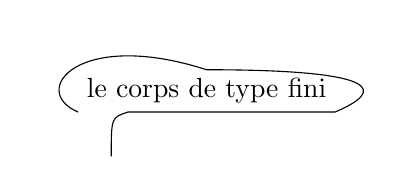
\begin{tikzpicture}[baseline=(n.base)]
\node[inner sep=3pt] (n) {le corps de type fini};
\draw (n.south west) .. controls ([xshift=-18pt]n.west) and ([yshift=15pt]n.north west) .. (n.north) .. controls ([xshift=18pt]n.north east) and ([xshift=18pt]n.east) .. (n.south east) -- ([xshift=18pt]n.south west) .. controls ([xshift=12pt,yshift=-2pt]n.south west) .. ([xshift=12pt,yshift=-16pt]n.south west);
\end{tikzpicture}}} $k_0$, et $k_0$ assez petit pour que $G_M$ connexe, mais \unsure{choisi} de degré de transcendance minimum, \deleted{alors si $\sigma\in\unsure{\operatorname{Aut}(k/k_0)}$ \unsure{tel que} $\sigma$ \unsure{de} \unsure{$M$} \unsure{fixe}} si $\sigma\in\deleted{\operatorname{Aut}_{k_0}k}\operatorname{Gal}(k/k_0)$
\margin{\figure{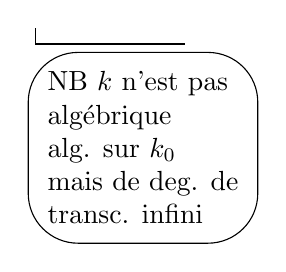
\begin{tikzpicture}
\draw (0.1,1.2)--(0.1,1)--(2,1);
\node[draw,rounded corners=18pt,align=left,inner sep=7pt,anchor=north west] at (0,0.9) {\uline{NB} $k$ n'est \uline{pas}\\\deleted{\unsure{algébrique}}\\\uline{alg. sur $k_0$}\\mais de deg. de\\transc. infini};
\end{tikzpicture}}}
on a
\[
M_{\sigma v}^{\mathbf Z}=\dot\sigma M_v^{\mathbf Z}
\]
où $\dot\sigma$ opère sur $M^{\mathbb A_{\unsure{c|C}}}$ \deleted{\unsure{en vertu}} de la façon suivante \deleted{\unsure{son image}}
\[
\dot\sigma\bigl((x_\ell)_{\ell\ \text{fini}},x_\infty\bigr)=(\sigma_\ell x_\ell,\dot\sigma_\infty x_\infty)
\]
où $\sigma_\ell$ provient de l'hom canonique
\[
\operatorname{Gal}(k/k_0)\mathbin{\text{---}}G(\mathbf Z_\ell),
\]
et $\dot\sigma_\infty$ est l'hom \uline{$\frac12$ linéaire} défini par $\sigma$ via
\[
\unsure{M_k|M_{/k}}(\infty)\simeq M_{k_0}(\infty)\otimes_{k_0}k.
\]
\mspage{52}

\scanpage{54}
\mspage{53}
2 - 5 - \hfill n° 392
\[
\begin{aligned}
(2)\qquad &\underline{ab}=\prod\underline p^{m(\underline p)+n(\underline p)}\\
(3)\qquad &\underline a:\underline b=\underline{ab}^{-1}=\prod\underline p^{m(\underline p)-n(\underline p)}\\
(4)\qquad &\underline a+\underline b=\prod\underline p^{\inf(m(\underline p),n(\underline p))}\\
(5)\qquad &\underline a\cap\underline b=\prod\underline p^{\sup(m(\underline p),n(\underline p))}.
\end{aligned}
\]
En effet, la relation (2) est évidente ; la relation (3) en résulte, l'égalité $\underline a:\underline b=\underline{ab}^{-1}$ découlant de la formule $\operatorname{div}(\underline a:\underline b)=\operatorname{div}\underline a-\operatorname{div}\underline b$, (§ 1, n° 2, cor. du th. 1) ; les formules (4) et (5) résultent de la prop. 2, § 1, n° 1.

Ces résultats s'appliquent notamment à la clôture intégrale de $Z$ dans une extension de degré fini de $Q$.

Lorsque $A$ est principal, les résultats ci-dessus redonnent ceux d'\uline{Alg.}, chap. VII, § 1, n° 3.

4. \uline{Théorème d'approximation dans les anneaux de Dedekind}.

Dans les anneaux de Dedekind, on a un ``théorème d'approximation'' qui améliore à la fois le th. 1 du chap. VI, § 7, n° 2 et la prop. 9 du § 1, n° 5 :

PROPOSITION 2.- \uline{Soient} $A$ \uline{un anneau de Dedekind}, $K$ \uline{son corps des fractions}, \uline{et} $P$ \uline{l'ensemble des idéaux premiers non nuls de} $A$ ; \uline{pour} $\underline p\in P$, \uline{notons} $v_{\underline p}$ \uline{la valuation essentielle correspondante de} $A$. \uline{Soient} $\underline p_1,\ldots,\underline p_q$ \uline{des éléments deux à deux distincts de} $P$, $n_1,\ldots,n_q$ \uline{des entiers rationnels}, \uline{et} $x_1,\ldots,x_q$ \uline{des éléments de} $K$. \uline{Il existe alors} $x\in K$ \uline{tel que} $v_{\underline p_i}(x-x_i)\ge n_i$ \uline{pour} $1\le i\le q$, \uline{et que} $v_{\underline p}(x)\ge0$ \uline{pour tout} $\underline p\in P$ \uline{distinct des} $\underline p_i$.

En remplaçant au besoin les $n_i$ par des entiers qui leurs sont supérieurs, on peut les supposer tous positifs. Examinons d'abord le cas où les $x_i$ sont dans $A$ ; tout revient évidemment à trouver un $x\in A$ vérifiant les congruences
\[
x\equiv x_i\ (\mathrm{mod.}\ \underline p^{n_i})
\]
et l'existence de $x$ résulte alors du chap. II, § 1, n° 2, prop. 5.

\scanpage{55}
Connaissant $v$ et $w$, on trouve donc \deleted{Donc} comme d'habitude qu'il existe un
\[
g\in G(\mathbb A_{\unsure{C|c}})=\prod_{\ell\ \mathrm{fini}}G(\mathbf Z_\ell)\times G(\mathbf C),
\]
tel que
\[
\deleted{\unsure{w=gv}}
\qquad M_w^{\deleted{\unsure{\mathbf Q}}\inserted{\mathbf Z}}=gM_v^{\deleted{\unsure{\mathbf Q}}\inserted{\mathbf Z}}
\]
où $G=G_{M\xi_v}$ est le grp alg. sur $\mathbf Q$ associé à $M,v$.

[\unsure{On vérifie|On considère} \unsure{que} les foncteurs $N\rightsquigarrow N_v^{\mathbf Z}$ et $N\rightsquigarrow N_w^{\mathbf Z}$ sur la catégorie des \uline{motifs} \uline{subordonnés} à $M$ sont isomorphes, \unsure{ce par considération par isomorphismes}]. D'ailleurs, $g$ est déterminé mod. multiplication à droite par $h\in G(\mathbf Z)$.
\inserted{$g\rightsquigarrow gh$ ($h\in G(\mathbf Z)$).}
\margin{N.B. Si on a fixé $g_\infty$ (ce qui est une indétermination mod $G(\mathbf Z)$ seulement) tous les $g_\ell$ sont déterminés.}

\deleted{Alors} On aura \inserted{\uline{en particulier}} pour $\sigma\in\operatorname{Gal}(k/k_0)$
\diagram{\begin{tikzcd}[ampersand replacement=\&,row sep=large]
\deleted{M_{\sigma w}^{\mathbf Z}=\dot\sigma(gM_v^{\mathbf Z})}\arrow[d]\\
M_{\sigma w}^{\mathbf Z}=\deleted{\unsure{g_\infty}}g_\sigma M_v^{\mathbf Z}\arrow[d,equal]\\
\sigma_\infty M_v^{\mathbf Z}
\end{tikzcd}}

\deleted{\margin{\figure{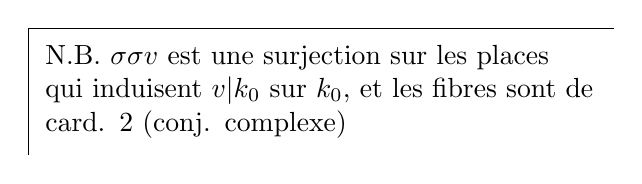
\begin{tikzpicture}
\node[align=left,text width=7cm,inner sep=6pt] (n) {N.B. $\sigma\rightsquigarrow\sigma v$ est une surjection sur les places qui induisent $v|k_0$ sur $k_0$, et les fibres sont de card. $2$ (conj. complexe)};
\draw (n.south west)--(n.north west)--(n.north east);
\end{tikzpicture}}}}
\deleted{donc on a une application
\diagram{\begin{tikzcd}[ampersand replacement=\&,column sep=large,execute at end picture={\draw ([xshift=-8pt,yshift=14pt]current bounding box.north west) rectangle ([xshift=8pt,yshift=-14pt]current bounding box.south east);}]
\operatorname{Gal}(k/k_0)\arrow[r,"\varphi_v"]\&G(\mathbb A_{\unsure{C|c}})/G(\mathbf Z)
\end{tikzcd}}
\[
M_{\sigma v}^{\mathbf Z}=\deleted{g_\sigma}\varphi_v(\sigma)M_v^{\mathbf Z}\quad\text{i.e.}\quad\dot\sigma_\infty(M_v^{\mathbf Z})=\varphi_v(\sigma)M_v^{\mathbf Z}
\]}
\mspage{54}

\scanpage{56}
\mspage{55}
2 - 4 - \hfill n° 392

$1\le i\le n$. Soit $x_0$ un élément de $K$ tel que $v_i(x_0)=q_i$ pour $1\le i\le n$, (chap. VI, § 7, n° 2, cor. 1 du th. 1). Alors $\underline a$ est l'ensemble des $x\in K$ tels que $v_i(xx_0^{-1})\ge0$ pour $1\le i\le n$. Ainsi $\underline a=Ax_0$.

Si $A$ est un anneau de Dedekind, on a vu, dans la démonstration du th. 1, que le groupe $D(A)$ des diviseurs de $A$ s'identifie au groupe $I(A)$ des idéaux fractionnaires $\underline a\ne(0)$, (comme $A$ est noethérien, tout idéal fractionnaire non nul est de type fini). Le groupe des \uline{classes de diviseurs} de $A$, (§ 1, n° 4), s'identifie alors au groupe des \uline{classes d'idéaux} de $A$, (chap. II, § 5, n° 7).

3. \uline{Décomposition des idéaux en produits d'idéaux premiers}.

Soient $A$ un anneau de Dedekind, $I(A)$ le groupe multiplicatif ordonné des idéaux fractionnaires non nuls de $A$, et $D(A)$ le groupe des diviseurs de $A$. L'isomorphisme $\underline a\longrightarrow\operatorname{div}\underline a$ de $I(A)$ sur $D(A)$ fait correspondre les diviseurs extrémaux aux idéaux premiers non nuls de $A$, (§ 1, n° 6, th. 3), donc le groupe multiplicatif $I(A)$ admet pour base l'ensemble des idéaux premiers non nuls de $A$, (§ 1, n° 3, th. 2). Autrement dit, \uline{tout idéal fractionnaire non nul} $\underline a$ \uline{de} $A$ \uline{admet une décomposition et une seule de la forme} :
\[
(1)\qquad\underline a=\prod\underline p^{n(\underline p)}
\]
où le produit est étendu aux idéaux premiers non nuls de $A$, les exposants $n(\underline p)$ étant nuls à l'exception d'un nombre fini d'entre eux. De plus $\underline a$ est entier si et seulement si les $n(\underline p)$ sont tous positifs. On dit que la relation (1) est la \uline{décomposition de} $\underline a$ \uline{en facteurs premiers}. En particulier, si $\underline a$ est un idéal principal $Ax$, on a, pour tout $\underline p$, $n(\underline p)=v_{\underline p}(x)$, où $v_{\underline p}$ désigne la valuation essentielle correspondant à $\underline p$ ; ceci résulte en effet de la formule (4) du § 1, n° 4. Soient
\[
\underline a=\prod\underline p^{m(\underline p)}\quad,\quad\underline b=\prod\underline p^{n(\underline p)}
\]
deux idéaux fractionnaires non nuls de $A$. On a alors :

\scanpage{57}
\deleted{Fixons un $v$ de référence (i.e. une topologie sur $k$, \unsure{déterm.} \unsure{isom.} $k\simeq\mathbf C$ mod conj. compl.).}

Or $g_\sigma$ est connu mod mult. à droite par $G(\mathbf Z)$, d'autre part $g_{\sigma\,\mathrm{fini}}$ est (avec la $=$ indétermination) le système des $\sigma_\ell$ galoisiens. Donc on peut prendre
\[
g_\sigma=((\deleted{g_\ell}\inserted{\sigma_\ell})_{\ell\ \mathrm{fini}},\sigma_\infty)
\]
\uline{où maintenant} $\sigma_\infty$ \uline{est un élément bien déterminé de} $G(\unsure{k|K})$ !!!

On obtient une application canonique
\diagram{\begin{tikzcd}[ampersand replacement=\&,column sep=large,execute at end picture={\draw ([xshift=-7pt,yshift=13pt]current bounding box.north west) rectangle ([xshift=-72pt,yshift=-13pt]current bounding box.south east);}]
\operatorname{Gal}(k/k_0)\arrow[r,"\varphi_v"]\&G_{\deleted{\unsure{\xi_v}}}(\unsure{k|K})\subset\mathrm{Gl}(M_k(\infty))
\end{tikzcd}}
\margin{\figure{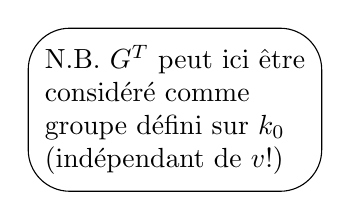
\begin{tikzpicture}\node[draw,rounded corners=15pt,align=left,inner sep=6pt] {N.B. $G^T$ peut ici être\\considéré comme\\groupe défini sur $k_0$\\(\uline{indépendant de $v$!})};\end{tikzpicture}}}
et telle qu'on ait
\diagram{\begin{tikzcd}[ampersand replacement=\&,column sep=small]
\dot\sigma M_v^{\mathbf Z}\arrow[r,equal]\&\left\{\begin{array}{l}M_{\sigma v}^{\mathbf Z}=\sigma_*M_v^{\mathbf Z}\qquad\text{pour }\sigma\in\operatorname{Gal}(k/k_0)\\[7pt]\sigma_*=((\sigma_\ell)_{\ell\ \mathrm{fini}},\varphi_v(\sigma)).\end{array}\right.
\end{tikzcd}}

On vérifie aussitôt
\[
\varphi_v(\tau\sigma)={}^\tau\varphi_v(\sigma)^{\deleted{\unsure{\tau|-1}}}\varphi_v(\tau)
\]
i.e. posant $\psi_v=\varphi_v^{-1}$
\[
\psi_v(\tau\sigma)=\psi_v(\tau){}^\tau\psi_v(\sigma)^{\deleted{\unsure{\tau|-1}}}
\]
\mspage{56}

\scanpage{58}
\mspage{57}
2 - 3 - \hfill n° 392

Montrons que c) implique d). Si c) est vraie, l'application $\underline a\longrightarrow\operatorname{div}\underline a$ est une bijection de $I(A)$ sur $D(A)$, (cf. § 1, n° 1) ; comme c'est un homomorphisme, (§ 1, n° 2), et que $D(A)$ est un groupe, tout élément de $I(A)$ est bien inversible.

Montrons que d) implique e). Si d) est vraie, tout idéal entier $\ne(0)$ de $A$ est de type fini, (chap. II, § 5, n° 6, th. 4), donc $A$ est noethérien ; comme $I(A)$ est un groupe, $D(A)$ est un groupe, et $A$ est donc complètement intégralement clos, (§ 1, n° 2, th. 1). Enfin, si $\underline p$ est un idéal premier non nul de $A$, et si $\underline m$ est un idéal maximal de $A$ contenant $\underline p$, l'anneau $A_{\underline m}$ est principal, (chap. II, § 5, n° 6, th. 4) ; comme $\underline pA_{\underline m}$ est premier non nul, on a nécessairement $\underline pA_{\underline m}=\underline mA_{\underline m}$, d'où $\underline p=\underline m$, (chap. II, § 2, n° 5, prop. 11), et $\underline p$ est maximal.

Montrons que e) implique f). En effet, si $\underline m$ est un idéal maximal de $A$, et si e) est vraie, $A_{\underline m}$ est un anneau noethérien intégralement clos, et son idéal maximal $\underline mA_{\underline m}$ est, ou bien $(0)$, ou bien le seul idéal premier non nul de $A_{\underline m}$ ; donc $A_{\underline m}$ est un corps ou un anneau de valuation discrète d'après la prop. 11 du § 1, n° 7.

Le fait que f) implique g) est évident.

Montrons enfin que g) implique a). Comme $A$ est l'intersection des $A_{\underline m}$, où $\underline m$ parcourt l'ensemble des idéaux maximaux, (chap. II, § 3, n° 3, cor. 4 du th. 1), g) implique que $A$ est intégralement clos et noethérien, donc que $A$ est un anneau de Krull, (§ 1, n° 3, cor. du th. 2). D'autre part, on montre que tout idéal premier non nul de $A$ est maximal comme dans la démonstration de d) $\Longrightarrow$ e). C. Q. F. D.

PROPOSITION 1.- \uline{Un anneau de Dedekind semi-local est principal}.

Soient $A$ un anneau de Dedekind semi-local, $K$ son corps des fractions, $p_1,\ldots,p_n$ ses idéaux maximaux, et $v_1,\ldots,v_n$ les valuations essentielles correspondantes ; ce sont les seules valuations essentielles de $A$. Soit $\underline a$ un idéal entier non nul de $A$. Puisqu'il est divisoriel, il existe, (§ 1, n° 4, prop. 5), des entiers $q_1,\ldots,q_n$ tels que $\underline a$ soit l'ensemble des $x\in K$ tels que $v_i(x)\ge q_i$ pour

\scanpage{59}
Ainsi $\unsure{\psi|\varphi}$ \uline{est un $1$-cocycle}, quand on fait opérer $\operatorname{Gal}(k/k_0)$ sur $G(k)$ de la façon évidente (par conjugaison). Il correspond à un fibré principal homogène $P_{v,k}$ sous $G(k)$, avec opérations de $\operatorname{Gal}(k/k_0)$ sur \deleted{$(P_v,G(k))$ compatibles avec le grp}. Il définit \inserted{par descente} un fibré principal homogène \inserted{$P_{v,k_0}$} sous $G_{k_0}$, avec un \uline{splitting donné} sur $k$.

On peut d'ailleurs dire ce que c'est que $P$ : c'est le fibré principal des isom \inserted{de foncteurs} $\xi_{M,\unsure{k_0|\infty}}$ avec $\xi_{M,v}^{\mathbf Z}\otimes_{\mathbf Z}k_0$, dont une trivialisation est en effet obtenue $\ldots$
\margin{\uline{À vérifier}\\OK.}

\unsure{Pour|Puis} la conjecture \inserted{de transcendance} N° 1, \deleted{\unsure{celle que l'hom}} \unsure{ce|le} point ainsi donné sur $P_{v,k}$ est \uline{générique}, revient à dire que l'application
\diagram{\begin{tikzcd}[ampersand replacement=\&,column sep=large]
\operatorname{Gal}(k/k_0)\arrow[r,"\varphi_v"]\&G(k)[\subset\mathrm{Gl}(M_k(\infty))]
\end{tikzcd}}
\deleted{est} a une image Zariski dense. [NB. elle l'est \unsure{déjà},
\margin{$\pi$ transcendant sur $k_0\ldots$}
\mspage{58}

\scanpage{60}
-VII- 19 - \hfill n° 383

\uline{Système de racines de type} $G_2$

\figure{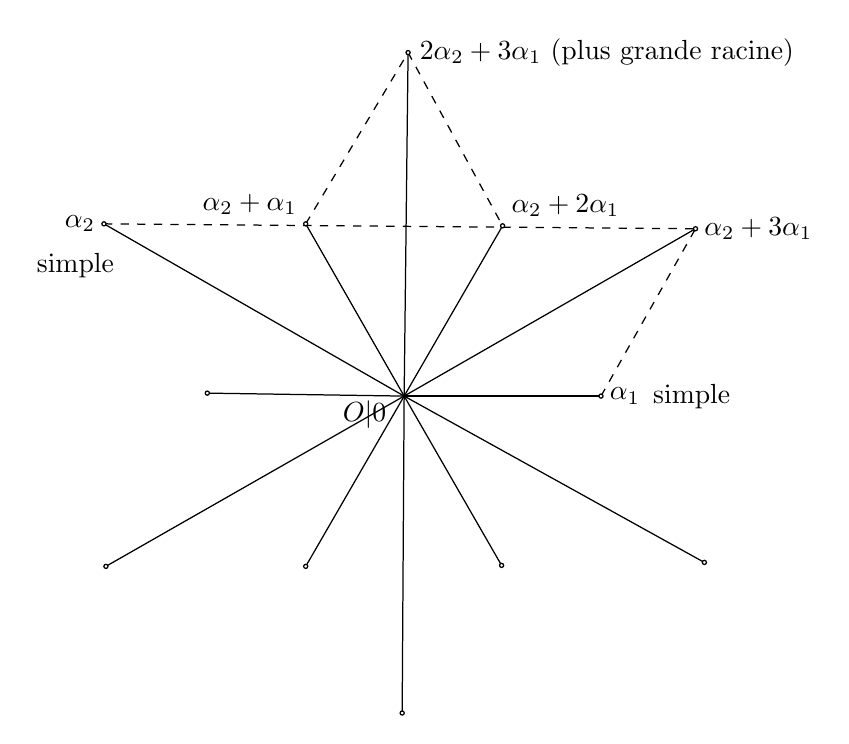
\begin{tikzpicture}[x=1.25cm,y=1.25cm,line width=.45pt]
\coordinate (O) at (0,0);
\coordinate (a) at (2,0);
\coordinate (b) at (-3.05,1.75);
\coordinate (c) at (-1,1.75);
\coordinate (d) at (1,1.73);
\coordinate (e) at (2.96,1.70);
\coordinate (f) at (.04,3.49);
\coordinate (na) at (-2,.03);
\coordinate (nb) at (3.05,-1.69);
\coordinate (nc) at (.99,-1.72);
\coordinate (nd) at (-1,-1.73);
\coordinate (ne) at (-3.03,-1.73);
\coordinate (nf) at (-.02,-3.22);
\draw[dashed] (b)--(e);
\draw[dashed] (c)--(f)--(d);
\draw[dashed] (a)--(e);
\foreach \p in {a,b,c,d,e,f,na,nb,nc,nd,ne,nf}{\draw (O)--(\p);\draw[fill=white] (\p) circle (.021);}
\node[below left,inner sep=2pt] at (-.12,.02) {$\unsure{O|0}$};
\node[right,inner sep=3pt] at (a) {$\alpha_1$};
\node[right] at (2.43,0) {simple};
\node[left,inner sep=3pt] at (b) {$\alpha_2$};
\node[below] at (-3.34,1.55) {simple};
\node[above left,inner sep=3pt] at (c) {$\alpha_2+\alpha_1$};
\node[above right,inner sep=3pt] at (d) {$\alpha_2+2\alpha_1$};
\node[right,inner sep=3pt] at (e) {$\alpha_2+3\alpha_1$};
\node[right,inner sep=4pt] at (f) {$2\alpha_2+3\alpha_1$ (plus grande racine)};
\end{tikzpicture}}
\mspage{59}

\scanpage{61}
quitte à passer à une extension finie de $k_0$, $\sigma_k\rightsquigarrow({}^\sigma g)^{-1}g$ \inserted{au lieu de $g^{-1}g^\sigma$} où $g\in G(\unsure{k|K})$ est gén. $(k_0)$.
\margin{(\unsure{$g$ n'est|$g$ est} déterminé mod mult par $g_0\in G(k_0)$)}
\figure{\begin{tikzpicture}[scale=.5]
\draw (0,0) .. controls (1,.35) and (2.1,.2) .. (2.4,.3) .. controls (4,.15) and (6,.3) .. (7,.3);
\draw[->] (2.4,-.7)--(2.4,.3);
\draw (7.1,.6) .. controls (7.1,1.15) and (8.5,1) .. (9.1,1.25);
\end{tikzpicture}}
On trouve alors que $g^\sigma$ \uline{\unsure{$\forall$|tt}} pt gén. de $G(k)$, et par suite $g^\sigma g^{-1}$ prend \deleted{\unsure{tt}} \inserted{\unsure{exactt}} les valeurs $a$ telles que $\deleted{g}ag$ soit gén. $/k_0$, par ex. \unsure{tts|ttes} valeurs telles que \deleted{$(\unsure{ag})$} \deleted{$ag$} $a$ soit gén. sur $k_0(g)$.

\deleted{En d'autres termes} Considérons enfin l'hom total $\sigma\longrightarrow\sigma_*$
\diagram{\begin{tikzcd}[ampersand replacement=\&,column sep=large]
\operatorname{Gal}(k/k_0)\arrow[r,"{\deleted{\unsure{\varphi_\infty}}\inserted{\varphi_v}}"]\&G(\mathbb A_{\unsure{C|c}})
\end{tikzcd}}
\deleted{\unsure{de dire} On a envie de dire que l'image}

Considérons le noyau de $\operatorname{Gal}(k/k_0)\mathbin{\text{---}}G(\mathbb A_{\mathrm{fin}})$, qui contient \unsure{le} noyau $\operatorname{Gal}(k/\bar k_0)$ de $\operatorname{Gal}(k/k_0)\mathbin{\text{---}}\operatorname{Gal}(\unsure{k/\bar k_0|\bar k_0/k_0})$. Ce noyau est envoyé dans $G(\mathbb A_{\unsure{C|c}})$ par $\varphi_{v\infty}$, et l'image est encore dense. \deleted{De façon plus précise,} \inserted{Il me semble que} \deleted{$\varphi_v$ est} \deleted{dominant} $\overline{\varphi_v(\operatorname{Gal}(k/k_0))}$ est un sous (\unsure{grps|gprs}) ouvert de $G(\mathbb A_{\unsure{C|c}})$.
\margin{\unsure{(1)?|( )?}}
\mspage{60}

\scanpage{62}
Cette application \unsure{peut|pour} \unsure{d'ailleurs} si $w'=\sigma w$
\margin{N.B. c'est \unsure{qu'une|ici une} petite vérification pour $w$\ldots\quad $v\to v'$.}
\[
M_w^{\mathbf Z}=gM_v^{\mathbf Z}
\]
\[
\begin{aligned}
M_{\sigma w}^{\mathbf Z}&=\dot\sigma(M_w^{\mathbf Z})=\dot\sigma gM_v^{\mathbf Z}
=\dot\sigma g\dot\sigma^{-1}(\dot\sigma M_v^{\mathbf Z})
=(\dot\sigma g\dot\sigma^{-1})\deleted{\unsure{\varphi_v}}\sigma_*M_v^{\mathbf Z}\\
&=\dot\sigma g\dot\sigma^{-1}\deleted{\unsure{\varphi_v}}\sigma_*\deleted{\unsure{g}}g^{-1}gM_v^{\mathbf Z}
\end{aligned}
\]
i.e.
\[
\left\{\begin{aligned}
M_{\sigma w}^{\mathbf Z}&=\deleted{\unsure{\varphi_w}}\sigma'_*M_w^{\mathbf Z}\\
\deleted{\varphi_w(\sigma)}&\deleted{=g^{\dot\sigma}\varphi_v(\sigma)g^{-1}}\\
\sigma'_*&=\dot\sigma g\dot\sigma^{-1}\sigma_*g^{-1}.
\end{aligned}\right.
\]
On a donc \inserted{pour $\ell$ fini}
\[
\sigma'_\ell=\sigma_\ell g_\ell\sigma_\ell^{-1}\sigma_\ell g_\ell^{-1}=\sigma_\ell
\]
d'où nécessairement
\[
\begin{aligned}
\sigma'_\infty&=\dot\sigma_\infty g_\infty\dot\sigma_\infty^{-1}\sigma_\infty g_\infty^{-1}\\
&=g_\infty^{\dot\sigma_\infty}\sigma_\infty g_\infty^{-1}.
\end{aligned}
\]
i.e. on a
\[
\deleted{\varphi_w(\sigma)=g_\infty^{\dot\sigma_\infty}\varphi_v(\sigma)g_\infty}
\]
\[
\left\{\begin{aligned}
&\boxed{\varphi_w(\sigma)=g_\infty^\sigma\varphi_v(\sigma)g_\infty^{-1}}\\
&\text{pour}\quad M_w^{\mathbf Z}=gM_v^{\mathbf Z},\quad g\in G\deleted{\unsure{k}}(M_k^{(\infty)})\\
&\text{i.e. si }w\text{ et }v\text{ sont }\uline{M\text{-équivalents}}.
\end{aligned}\right.
\]
\mspage{61}
